\documentclass[11pt,a4paper]{article}
\usepackage[utf8]{inputenc}
\usepackage[T1]{fontenc}
\usepackage{lmodern}
\usepackage{textcomp}
\usepackage{amsmath,amssymb}
\usepackage{graphicx}
\usepackage{booktabs}
\usepackage{longtable}
\usepackage{array}
\usepackage{listings}
\usepackage{xcolor}
\usepackage[margin=1in]{geometry}
\usepackage{float}
\usepackage[hidelinks,breaklinks]{hyperref}
\usepackage{microtype}
\setlength{\parskip}{4pt}
\lstset{basicstyle=\ttfamily\scriptsize,breaklines=true,breakatwhitespace=false,
  postbreak=\mbox{\textcolor{gray}{$\hookrightarrow$}\space},frame=single,
  framerule=0.3pt,rulecolor=\color{gray!60},columns=fullflexible,keepspaces=true,
  showstringspaces=false,numbers=none,xleftmargin=4pt,xrightmargin=4pt,
  literate={\_}{{\_}}1}
\graphicspath{{figures/}}
\providecommand{\tightlist}{}
\title{Supplementary material: Lyman-alpha Warm Dark Matter Limits Compared with Dodelson-Widrow Sterile-Neutrino Production Fractions}
\author{HEP-Genesis-Agent session record \\ \small Project: ramp-research-lyman-wdm}
\date{2026-10-19}
\begin{document}
\maketitle
\noindent\textit{\small Supplementary material, generated mechanically from the session record: it lists exactly what ran, in order, without interpretation.}
\vspace{1em}



\appendix
\section{Implementation details}
\label{app:impl}
This appendix is generated mechanically from the session record; it lists exactly what ran, in order, without interpretation.
\subsection{Session}
\begin{itemize}
  \item Source: cli client; conversation \texttt{a4887127}
  \item Started: 2026-10-19 11:01:20; report generated: 2026-10-19 11:13:14
  \item Project: ramp-research-lyman-wdm (\texttt{/\allowbreak{}Users/\allowbreak{}nramachandra/\allowbreak{}hep-genesis-testing/\allowbreak{}projects/\allowbreak{}ramp-research-lyman-wdm})
  \item Compute execution site(s) selected in the session: local
  \item 1 user turn(s), 104 tool call(s) (0 returned errors), 15 figure(s), 17 data file(s)
\end{itemize}
\subsection{Models}
\begin{longtable}{@{}p{0.16\textwidth}p{0.34\textwidth}p{0.44\textwidth}@{}}
\toprule Stage & Model & Endpoint \\ \midrule \endhead
quick & \texttt{claude-opus-5-5} & \texttt{https:\allowbreak{}/\allowbreak{}/\allowbreak{}mag.genesis.americansciencecloud.org/\allowbreak{}v1} \\
report & \texttt{claude-opus-5-5} & \texttt{https:\allowbreak{}/\allowbreak{}/\allowbreak{}mag.genesis.americansciencecloud.org/\allowbreak{}v1} \\
coder & \texttt{claude-opus-5-5} & \texttt{https:\allowbreak{}/\allowbreak{}/\allowbreak{}mag.genesis.americansciencecloud.org/\allowbreak{}v1} \\
\bottomrule\end{longtable}
\subsection{MCP servers}
\begin{longtable}{@{}p{0.22\textwidth}p{0.12\textwidth}p{0.6\textwidth}@{}}
\toprule Server & Transport & Location \\ \midrule \endhead
hep-research-aid & stdio & \texttt{python -m hep\_\allowbreak{}genesis.domain.mcp\_\allowbreak{}server} \\
alcf-tools & stdio & \texttt{python -m hep\_\allowbreak{}genesis.iri.alcf.mcp\_\allowbreak{}server} \\
nersc-tools & stdio & \texttt{python -m hep\_\allowbreak{}genesis.iri.nersc.mcp\_\allowbreak{}server} \\
\bottomrule\end{longtable}
\subsection{Tool-call log}
Chronological; arguments and results are truncated for space (the full record is in the project's \texttt{provenance/} folder).
\begin{longtable}{@{}p{0.04\textwidth}p{0.22\textwidth}p{0.36\textwidth}p{0.32\textwidth}@{}}
\toprule \# & Tool & Arguments & Outcome \\ \midrule \endhead
1 & \texttt{hep-research-aid}\newline\texttt{list\_\allowbreak{}agent\_\allowbreak{}files} & \texttt{\{\}\allowbreak{}} & \texttt{[]\allowbreak{}} \\
2 & \texttt{hep-research-aid}\newline\texttt{list\_\allowbreak{}input\_\allowbreak{}files} & \texttt{\{\}\allowbreak{}} & \texttt{\{   ''status'':\allowbreak{} ''success'',\allowbreak{}   ''files'':\allowbreak{} []\allowbreak{},\allowbreak{}   ''usage'':\allowbreak{} ''Pass any of these filenames to load\_\allowbreak{}table\_\allowbreak{}data()\allowbreak{}.'' \}\allowbreak{}} \\
3 & \texttt{hep-research-aid}\newline\texttt{list\_\allowbreak{}datasets} & \texttt{\{\}\allowbreak{}} & \texttt{\{'count':\allowbreak{} 0,\allowbreak{} 'datasets':\allowbreak{} []\allowbreak{}\}\allowbreak{}} \\
4 & \texttt{hep-research-aid}\newline\texttt{list\_\allowbreak{}files} & \texttt{\{\}\allowbreak{}} & \texttt{Files in .:\allowbreak{}   - .git   - .gitignore   - ISSUES.md   - SCOPE.md   - docs   - downloads   - logs   - projects   - reports   - research-results   - runs   - scripts   - venvs   - workspace} \\
5 & \texttt{hep-research-aid}\newline\texttt{get\_\allowbreak{}dispatch} & \texttt{\{\}\allowbreak{}} & \texttt{Dispatch:\allowbreak{} local execution.} \\
6 & \texttt{serve-sbbn.sh}\newline\texttt{list\_\allowbreak{}sterile\_\allowbreak{}nu\_\allowbreak{}skills} & \texttt{\{\}\allowbreak{}} & \texttt{\{   ''status'':\allowbreak{} ''ok'',\allowbreak{}   ''files'':\allowbreak{} []\allowbreak{},\allowbreak{}   ''message'':\allowbreak{} ''2 skills. Load one with load\_\allowbreak{}sterile\_\allowbreak{}nu\_\allowbreak{}skill.'',\allowbreak{}   ''metadata'':\allowbreak{} \{     ''skills'':\allowbreak{} \{       ''kev-sterile-dm-xray'':\allowbreak{} ''keV sterile-neutrino dark matter \textbackslash{}\allowbreak{}u2014 \ldots{}\allowbreak{}} \\
7 & \texttt{local}\newline\texttt{search\_\allowbreak{}arxiv\_\allowbreak{}abstracts} & \texttt{\{''query'':\allowbreak{} ''Lyman-alpha forest warm dark matter thermal relic mass lower limit'',\allowbreak{} ''max\_\allowbreak{}results'':\allowbreak{} 8\}\allowbreak{}} & \texttt{[1107.3837v2]\allowbreak{} The Lyman-alpha forest in a blazar-heated Universe Abstract:\allowbreak{} It has been realised only recently that TeV emission from blazars can significantly heat the intergalactic medium (IGM)\allowbreak{} by pa\ldots{}\allowbreak{}} \\
8 & \texttt{local}\newline\texttt{search\_\allowbreak{}arxiv\_\allowbreak{}abstracts} & \texttt{\{''query'':\allowbreak{} ''non-resonant Dodelson-Widrow sterile neutrino Lyman-alpha constraint mapping thermal relic'',\allowbreak{} ''max\_\allowbreak{}results'':\allowbreak{} 6\}\allowbreak{}} & \texttt{[0507333v2]\allowbreak{} UHE neutrino damping in a thermal gas of relic neutrinos Abstract:\allowbreak{}   We present a calculation of the damping of an ultra-energetic (UHE)\allowbreak{} cosmic neutrino travelling through the thermal gas \ldots{}\allowbreak{}} \\
9 & \texttt{local}\newline\texttt{search\_\allowbreak{}arxiv\_\allowbreak{}abstracts} & \texttt{\{''query'':\allowbreak{} ''Viel 2013 warm dark matter HIRES MIKE Lyman-alpha'',\allowbreak{} ''max\_\allowbreak{}results'':\allowbreak{} 4\}\allowbreak{}} & \texttt{[0812.0010v2]\allowbreak{} Lyman-alpha constraints on warm and on warm-plus-cold dark matter models Abstract:\allowbreak{}   We revisit Lyman-alpha bounds on the dark matter mass in Lambda Warm Dark Matter (Lambda-WDM)\allowbreak{} models,\allowbreak{}\ldots{}\allowbreak{}} \\
10 & \texttt{local}\newline\texttt{search\_\allowbreak{}arxiv\_\allowbreak{}abstracts} & \texttt{\{''max\_\allowbreak{}results'':\allowbreak{} 6,\allowbreak{} ''query'':\allowbreak{} ''Lyman-alpha forest high-resolution new constraints warm dark matter 2023 Irsic thermal history''\}\allowbreak{}} & \texttt{[1107.3837v2]\allowbreak{} The Lyman-alpha forest in a blazar-heated Universe Abstract:\allowbreak{} It has been realised only recently that TeV emission from blazars can significantly heat the intergalactic medium (IGM)\allowbreak{} by pa\ldots{}\allowbreak{}} \\
11 & \texttt{local}\newline\texttt{search\_\allowbreak{}arxiv\_\allowbreak{}abstracts} & \texttt{\{''max\_\allowbreak{}results'':\allowbreak{} 6,\allowbreak{} ''query'':\allowbreak{} ''Villasenor thermal relic dark matter Lyman-alpha inhomogeneous reionization 2022''\}\allowbreak{}} & \texttt{[9902180v2]\allowbreak{} Scattered Lyman-alpha Radiation Around Sources Before Cosmological Reionization Abstract:\allowbreak{}   The spectra of the first galaxies and quasars in the Universe should be strongly absorbed shortw\ldots{}\allowbreak{}} \\
12 & \texttt{local}\newline\texttt{search\_\allowbreak{}arxiv\_\allowbreak{}abstracts} & \texttt{\{''max\_\allowbreak{}results'':\allowbreak{} 6,\allowbreak{} ''query'':\allowbreak{} ''eBOSS Lyman-alpha hints neutrino masses warm dark matter Palanque-Delabrouille''\}\allowbreak{}} & \texttt{[1506.05976v3]\allowbreak{} Neutrino masses and cosmology with Lyman-alpha forest power spectrum Abstract:\allowbreak{} We present constraints on neutrino masses,\allowbreak{} the primordial fluctuation spectrum from inflation,\allowbreak{} and other p\ldots{}\allowbreak{}} \\
13 & \texttt{hep-research-aid}\newline\texttt{search\_\allowbreak{}arxiv} & \texttt{\{''query'':\allowbreak{} ''warm dark matter Lyman-alpha forest constraints 5.3 keV thermal relic'',\allowbreak{} ''max\_\allowbreak{}results'':\allowbreak{} 6\}\allowbreak{}} & \texttt{Found 6 papers matching query:\allowbreak{} 'warm dark matter Lyman-alpha forest constraints 5.3 keV thermal relic' (source:\allowbreak{} arXiv API)\allowbreak{}  Paper 1:\allowbreak{} arXiv ID:\allowbreak{} 1107.3837v2 Title:\allowbreak{} The Lyman-alpha forest in a blazar-hea\ldots{}\allowbreak{}} \\
14 & \texttt{hep-research-aid}\newline\texttt{search\_\allowbreak{}arxiv} & \texttt{\{''query'':\allowbreak{} ''sterile neutrino dark matter momentum distribution Dodelson-Widrow transfer function structure formation bounds'',\allowbreak{} ''max\_\allowbreak{}results'':\allowbreak{} 6\}\allowbreak{}} & \texttt{Found 6 papers matching query:\allowbreak{} 'sterile neutrino dark matter momentum distribution Dodelson-Widrow transfer function structure formation bounds' (source:\allowbreak{} arXiv API)\allowbreak{}  Paper 1:\allowbreak{} arXiv ID:\allowbreak{} 1702.08430v1 Ti\ldots{}\allowbreak{}} \\
15 & \texttt{local}\newline\texttt{web\_\allowbreak{}search} & \texttt{\{''query'':\allowbreak{} ''Villasenor 2022 new constraints warm dark matter Lyman-alpha forest inhomogeneous reionization arXiv''\}\allowbreak{}} & \texttt{We present new constraints on models of dark matter interacting with neutrino,\allowbreak{} based on high-resolution Lyman-\$$\alpha$\$ forest data. We perform a suite of full hydrodynamical simulations of these models,\allowbreak{} sp\ldots{}\allowbreak{}} \\
16 & \texttt{local}\newline\texttt{get\_\allowbreak{}arxiv\_\allowbreak{}metadata} & \texttt{\{''arxiv\_\allowbreak{}id'':\allowbreak{} ''2309.04533''\}\allowbreak{}} & \texttt{arXiv ID:\allowbreak{} 2309.04533 Title:\allowbreak{} Unveiling Dark Matter free-streaming at the smallest scales with high redshift Lyman-alpha forest Authors:\allowbreak{} Vid Ir?i?,\allowbreak{} Matteo Viel,\allowbreak{} Martin G. Haehnelt,\allowbreak{} James S. Bolton,\allowbreak{} Marg\ldots{}\allowbreak{}} \\
17 & \texttt{local}\newline\texttt{get\_\allowbreak{}arxiv\_\allowbreak{}metadata} & \texttt{\{''arxiv\_\allowbreak{}id'':\allowbreak{} ''1306.2314''\}\allowbreak{}} & \texttt{arXiv ID:\allowbreak{} 1306.2314 Title:\allowbreak{} Warm Dark Matter as a solution to the small scale crisis:\allowbreak{} new constraints from high redshift Lyman-alpha forest data Authors:\allowbreak{} M. Viel,\allowbreak{} G. D. Becker,\allowbreak{} J. S. Bolton,\allowbreak{} M. G. Haeh\ldots{}\allowbreak{}} \\
18 & \texttt{local}\newline\texttt{get\_\allowbreak{}arxiv\_\allowbreak{}metadata} & \texttt{\{''arxiv\_\allowbreak{}id'':\allowbreak{} ''2209.14220''\}\allowbreak{}} & \texttt{arXiv ID:\allowbreak{} 2209.14220 Title:\allowbreak{} New Constraints on Warm Dark Matter from the Lyman-\$$\alpha$\$ Forest Power Spectrum Authors:\allowbreak{} Bruno Villasenor,\allowbreak{} Brant Robertson,\allowbreak{} Piero Madau,\allowbreak{} Evan Schneider Year:\allowbreak{} 2022 Abstract:\allowbreak{} Th\ldots{}\allowbreak{}} \\
19 & \texttt{serve-sbbn.sh}\newline\texttt{describe\_\allowbreak{}sterile\_\allowbreak{}nu\_\allowbreak{}tools} & \texttt{\{\}\allowbreak{}} & \texttt{\{   ''status'':\allowbreak{} ''ok'',\allowbreak{}   ''files'':\allowbreak{} []\allowbreak{},\allowbreak{}   ''message'':\allowbreak{} ''Sterile Neutrino -\textgreater{}\allowbreak{} BBN /\allowbreak{} X-ray Bridge Server\textbackslash{}\allowbreak{}n=\allowbreak{}=\allowbreak{}=\allowbreak{}=\allowbreak{}=\allowbreak{}=\allowbreak{}=\allowbreak{}=\allowbreak{}=\allowbreak{}=\allowbreak{}=\allowbreak{}=\allowbreak{}=\allowbreak{}=\allowbreak{}=\allowbreak{}=\allowbreak{}=\allowbreak{}=\allowbreak{}=\allowbreak{}=\allowbreak{}=\allowbreak{}=\allowbreak{}=\allowbreak{}=\allowbreak{}=\allowbreak{}=\allowbreak{}=\allowbreak{}=\allowbreak{}=\allowbreak{}=\allowbreak{}=\allowbreak{}=\allowbreak{}=\allowbreak{}=\allowbreak{}=\allowbreak{}=\allowbreak{}=\allowbreak{}=\allowbreak{}=\allowbreak{}=\allowbreak{}=\allowbreak{}=\allowbreak{}=\allowbreak{}=\allowbreak{}=\allowbreak{}\textbackslash{}\allowbreak{}n\textbackslash{}\allowbreak{}nMaps sterile-neutrino particle parameters (m\_\allowbreak{}s,\allowbreak{} sin\textasciicircum{}\allowbreak{}2 2\ldots{}\allowbreak{}} \\
20 & \texttt{serve-sbbn.sh}\newline\texttt{list\_\allowbreak{}sterile\_\allowbreak{}nu\_\allowbreak{}skills} & \texttt{\{\}\allowbreak{}} & \texttt{\{   ''status'':\allowbreak{} ''ok'',\allowbreak{}   ''files'':\allowbreak{} []\allowbreak{},\allowbreak{}   ''message'':\allowbreak{} ''2 skills. Load one with load\_\allowbreak{}sterile\_\allowbreak{}nu\_\allowbreak{}skill.'',\allowbreak{}   ''metadata'':\allowbreak{} \{     ''skills'':\allowbreak{} \{       ''kev-sterile-dm-xray'':\allowbreak{} ''keV sterile-neutrino dark matter \textbackslash{}\allowbreak{}u2014 \ldots{}\allowbreak{}} \\
21 & \texttt{serve-sbbn.sh}\newline\texttt{load\_\allowbreak{}sterile\_\allowbreak{}nu\_\allowbreak{}skill} & \texttt{\{''name'':\allowbreak{} ''kev-sterile-dm-xray''\}\allowbreak{}} & \texttt{\{   ''status'':\allowbreak{} ''ok'',\allowbreak{}   ''files'':\allowbreak{} []\allowbreak{},\allowbreak{}   ''message'':\allowbreak{} ''Loaded skill 'kev-sterile-dm-xray'. Follow these instructions.'',\allowbreak{}   ''metadata'':\allowbreak{} \{     ''instructions'':\allowbreak{} ''---\textbackslash{}\allowbreak{}nname:\allowbreak{} kev-sterile-dm-xray\textbackslash{}\allowbreak{}ndescription:\allowbreak{} keV \ldots{}\allowbreak{}} \\
22 & \texttt{serve-sbbn.sh}\newline\texttt{predict\_\allowbreak{}sterile\_\allowbreak{}nu} & \texttt{\{''m\_\allowbreak{}s\_\allowbreak{}eV'':\allowbreak{} 7100,\allowbreak{} ''sin2\_\allowbreak{}2theta'':\allowbreak{} 7e-11\}\allowbreak{}} & \texttt{\{   ''status'':\allowbreak{} ''ok'',\allowbreak{}   ''files'':\allowbreak{} []\allowbreak{},\allowbreak{}   ''message'':\allowbreak{} ''Sterile neutrino:\allowbreak{} m\_\allowbreak{}s =\allowbreak{} 7.1e+03 eV,\allowbreak{} sin\textbackslash{}\allowbreak{}u00b22\textbackslash{}\allowbreak{}u03b8 =\allowbreak{} 7e-11\textbackslash{}\allowbreak{}nMechanism:\allowbreak{} DW\textbackslash{}\allowbreak{}n\textbackslash{}\allowbreak{}n\textbackslash{}\allowbreak{}u2500\textbackslash{}\allowbreak{}u2500 What the sterile \textbackslash{}\allowbreak{}u03bd produces \textbackslash{}\allowbreak{}u2500\textbackslash{}\allowbreak{}u2500\textbackslash{}\allowbreak{}n\textbackslash{}\allowbreak{}u0394N\_\allowbreak{}eff \ldots{}\allowbreak{}} \\
23 & \texttt{local}\newline\texttt{search\_\allowbreak{}arxiv\_\allowbreak{}abstracts} & \texttt{\{''query'':\allowbreak{} ''NuSTAR blank sky sterile neutrino dark matter decay line limits mixing angle'',\allowbreak{} ''max\_\allowbreak{}results'':\allowbreak{} 8\}\allowbreak{}} & \texttt{[1606.02684v1]\allowbreak{} Neutrino Oscillations With Two Sterile Neutrinos Abstract:\allowbreak{} This work estimates the probability of \$$\mu$\$ to \$e\$ neutrino oscillation with two sterile neutrinos using a 5x5 U-matrix,\allowbreak{} an ext\ldots{}\allowbreak{}} \\
24 & \texttt{local}\newline\texttt{download\_\allowbreak{}arxiv\_\allowbreak{}full\_\allowbreak{}text} & \texttt{\{''arxiv\_\allowbreak{}id'':\allowbreak{} ''2309.04533'',\allowbreak{} ''output\_\allowbreak{}dir'':\allowbreak{} ''/\allowbreak{}Users/\allowbreak{}nramachandra/\allowbreak{}hep-genesis-testing/\allowbreak{}projects/\allowbreak{}ramp-research-lyman-wdm/\allowbreak{}runs/\allowbreak{}261019\_\allowbreak{}110120''\}\allowbreak{}} & \texttt{Downloaded:\allowbreak{} /\allowbreak{}Users/\allowbreak{}nramachandra/\allowbreak{}hep-genesis-testing/\allowbreak{}projects/\allowbreak{}ramp-research-lyman-wdm/\allowbreak{}runs/\allowbreak{}261019\_\allowbreak{}110120/\allowbreak{}2309.04533.txt} \\
25 & \texttt{serve-sbbn.sh}\newline\texttt{predict\_\allowbreak{}sterile\_\allowbreak{}nu\_\allowbreak{}grid} & \texttt{\{''masses\_\allowbreak{}eV'':\allowbreak{} [1000,\allowbreak{} 1500,\allowbreak{} 2000,\allowbreak{} 3000,\allowbreak{} 5000,\allowbreak{} 7100,\allowbreak{} 10000,\allowbreak{} 15000,\allowbreak{} 20000,\allowbreak{} 22000,\allowbreak{} 25000,\allowbreak{} 29000,\allowbreak{} 35000,\allowbreak{} 45000,\allowbreak{} 60000,\allowbreak{} 80000,\allowbreak{} 100000]\allowbreak{},\allowbreak{} ''sin2\_\allowbreak{}2thetas'':\allowbreak{} [1e-13,\allowbreak{} 2.154e-13,\allowbreak{} 4.642e-13,\allowbreak{} 1e-12,\allowbreak{} 2.154e-12,\allowbreak{} 4.642e-12,\allowbreak{} 1e-11,\allowbreak{} 2.154e-1\ldots{}\allowbreak{}} & \texttt{\{   ''status'':\allowbreak{} ''ok'',\allowbreak{}   ''files'':\allowbreak{} [     ''/\allowbreak{}Users/\allowbreak{}nramachandra/\allowbreak{}hep-genesis-testing/\allowbreak{}projects/\allowbreak{}ramp-research-lyman-wdm/\allowbreak{}runs/\allowbreak{}261019\_\allowbreak{}110120/\allowbreak{}sterile\_\allowbreak{}nu\_\allowbreak{}grid\_\allowbreak{}DW\_\allowbreak{}4bbf6a.csv''   ]\allowbreak{},\allowbreak{}   ''message'':\allowbreak{} ''Predicted 374 points\ldots{}\allowbreak{}} \\
26 & \texttt{local}\newline\texttt{get\_\allowbreak{}arxiv\_\allowbreak{}metadata} & \texttt{\{''arxiv\_\allowbreak{}id'':\allowbreak{} ''1702.08430''\}\allowbreak{}} & \texttt{arXiv ID:\allowbreak{} 1702.08430 Title:\allowbreak{} keV sterile neutrino Dark Matter Authors:\allowbreak{} Alexander Merle Year:\allowbreak{} 2017 Abstract:\allowbreak{} We give an overview of the current status of keV sterile neutrino Dark Matter. After a short \ldots{}\allowbreak{}} \\
27 & \texttt{hep-research-aid}\newline\texttt{read\_\allowbreak{}text\_\allowbreak{}file} & \texttt{\{''filepath'':\allowbreak{} ''/\allowbreak{}Users/\allowbreak{}nramachandra/\allowbreak{}hep-genesis-testing/\allowbreak{}projects/\allowbreak{}ramp-research-lyman-wdm/\allowbreak{}runs/\allowbreak{}261019\_\allowbreak{}110120/\allowbreak{}sterile\_\allowbreak{}nu\_\allowbreak{}grid\_\allowbreak{}DW\_\allowbreak{}4bbf6a.csv''\}\allowbreak{}} & \texttt{m\_\allowbreak{}s\_\allowbreak{}eV,\allowbreak{}sin2\_\allowbreak{}2theta,\allowbreak{}delta\_\allowbreak{}neff,\allowbreak{}neff,\allowbreak{}omega\_\allowbreak{}s\_\allowbreak{}h2,\allowbreak{}Yp,\allowbreak{}DH\_\allowbreak{}x1e5,\allowbreak{}Li7H\_\allowbreak{}x1e10,\allowbreak{}chi2\_\allowbreak{}bbn,\allowbreak{}delta\_\allowbreak{}chi2\_\allowbreak{}bbn,\allowbreak{}lifetime\_\allowbreak{}s,\allowbreak{}free\_\allowbreak{}streaming\_\allowbreak{}kpc,\allowbreak{}bbn\_\allowbreak{}excluded\_\allowbreak{}95,\allowbreak{}overcloses,\allowbreak{}bbn\_\allowbreak{}treatment\_\allowbreak{}valid 1000,\allowbreak{}1e-13,\allowbreak{}1.28919e-07,\allowbreak{}3.044,\allowbreak{}1.\ldots{}\allowbreak{}} \\
28 & \texttt{local}\newline\texttt{download\_\allowbreak{}arxiv\_\allowbreak{}full\_\allowbreak{}text} & \texttt{\{''arxiv\_\allowbreak{}id'':\allowbreak{} ''2504.06367'',\allowbreak{} ''output\_\allowbreak{}dir'':\allowbreak{} ''/\allowbreak{}Users/\allowbreak{}nramachandra/\allowbreak{}hep-genesis-testing/\allowbreak{}projects/\allowbreak{}ramp-research-lyman-wdm/\allowbreak{}runs/\allowbreak{}261019\_\allowbreak{}110120''\}\allowbreak{}} & \texttt{Downloaded:\allowbreak{} /\allowbreak{}Users/\allowbreak{}nramachandra/\allowbreak{}hep-genesis-testing/\allowbreak{}projects/\allowbreak{}ramp-research-lyman-wdm/\allowbreak{}runs/\allowbreak{}261019\_\allowbreak{}110120/\allowbreak{}2504.06367.txt} \\
29 & \texttt{serve-sbbn.sh}\newline\texttt{predict\_\allowbreak{}sterile\_\allowbreak{}nu\_\allowbreak{}grid} & \texttt{\{''masses\_\allowbreak{}eV'':\allowbreak{} [7100,\allowbreak{} 10000,\allowbreak{} 15000,\allowbreak{} 20000,\allowbreak{} 22000,\allowbreak{} 25000,\allowbreak{} 29000,\allowbreak{} 35000,\allowbreak{} 45000,\allowbreak{} 60000,\allowbreak{} 80000,\allowbreak{} 100000]\allowbreak{},\allowbreak{} ''sin2\_\allowbreak{}2thetas'':\allowbreak{} [1e-12]\allowbreak{},\allowbreak{} ''mechanism'':\allowbreak{} ''DW'',\allowbreak{} ''output\_\allowbreak{}dir'':\allowbreak{} ''/\allowbreak{}Users/\allowbreak{}nramachandra/\allowbreak{}hep-genesis-testing/\allowbreak{}projects/\allowbreak{}ramp-researc\ldots{}\allowbreak{}} & \texttt{\{   ''status'':\allowbreak{} ''ok'',\allowbreak{}   ''files'':\allowbreak{} [     ''/\allowbreak{}Users/\allowbreak{}nramachandra/\allowbreak{}hep-genesis-testing/\allowbreak{}projects/\allowbreak{}ramp-research-lyman-wdm/\allowbreak{}runs/\allowbreak{}261019\_\allowbreak{}110120/\allowbreak{}sterile\_\allowbreak{}nu\_\allowbreak{}grid\_\allowbreak{}DW\_\allowbreak{}a74034.csv''   ]\allowbreak{},\allowbreak{}   ''message'':\allowbreak{} ''Predicted 12 points \ldots{}\allowbreak{}} \\
30 & \texttt{local}\newline\texttt{search\_\allowbreak{}arxiv\_\allowbreak{}abstracts} & \texttt{\{''max\_\allowbreak{}results'':\allowbreak{} 6,\allowbreak{} ''query'':\allowbreak{} ''Roach NuSTAR blank-sky sterile neutrino dark matter constraints 2022''\}\allowbreak{}} & \texttt{[1702.08430v1]\allowbreak{} keV sterile neutrino Dark Matter Abstract:\allowbreak{} We give an overview of the current status of keV sterile neutrino Dark Matter. After a short introduction,\allowbreak{} we start by a general discussion of\ldots{}\allowbreak{}} \\
31 & \texttt{local}\newline\texttt{download\_\allowbreak{}arxiv\_\allowbreak{}full\_\allowbreak{}text} & \texttt{\{''arxiv\_\allowbreak{}id'':\allowbreak{} ''0812.0010'',\allowbreak{} ''output\_\allowbreak{}dir'':\allowbreak{} ''/\allowbreak{}Users/\allowbreak{}nramachandra/\allowbreak{}hep-genesis-testing/\allowbreak{}projects/\allowbreak{}ramp-research-lyman-wdm/\allowbreak{}runs/\allowbreak{}261019\_\allowbreak{}110120''\}\allowbreak{}} & \texttt{Downloaded:\allowbreak{} /\allowbreak{}Users/\allowbreak{}nramachandra/\allowbreak{}hep-genesis-testing/\allowbreak{}projects/\allowbreak{}ramp-research-lyman-wdm/\allowbreak{}runs/\allowbreak{}261019\_\allowbreak{}110120/\allowbreak{}0812.0010.txt} \\
32 & \texttt{serve-sbbn.sh}\newline\texttt{predict\_\allowbreak{}sterile\_\allowbreak{}nu\_\allowbreak{}xray\_\allowbreak{}line} & \texttt{\{''m\_\allowbreak{}s\_\allowbreak{}eV'':\allowbreak{} 20000,\allowbreak{} ''sin2\_\allowbreak{}2theta'':\allowbreak{} 3.95e-11\}\allowbreak{}} & \texttt{\{   ''status'':\allowbreak{} ''ok'',\allowbreak{}   ''files'':\allowbreak{} []\allowbreak{},\allowbreak{}   ''message'':\allowbreak{} ''X-ray line prediction for Perseus,\allowbreak{} M31,\allowbreak{} Milky\_\allowbreak{}Way\_\allowbreak{}center,\allowbreak{} Coma,\allowbreak{} stacked\_\allowbreak{}galaxies\textbackslash{}\allowbreak{}nm\_\allowbreak{}s =\allowbreak{} 20 keV,\allowbreak{} sin\textbackslash{}\allowbreak{}u00b22\textbackslash{}\allowbreak{}u03b8 =\allowbreak{} 3.9e-11\textbackslash{}\allowbreak{}n\textbackslash{}\allowbreak{}nE\_\allowbreak{}\textbackslash{}\allowbreak{}u03b3 =\allowbreak{} 10 keV\textbackslash{}\allowbreak{}nDecay \ldots{}\allowbreak{}} \\
33 & \texttt{serve-sbbn.sh}\newline\texttt{predict\_\allowbreak{}sterile\_\allowbreak{}nu\_\allowbreak{}xray\_\allowbreak{}line} & \texttt{\{''m\_\allowbreak{}s\_\allowbreak{}eV'':\allowbreak{} 45000,\allowbreak{} ''sin2\_\allowbreak{}2theta'':\allowbreak{} 9.17e-12\}\allowbreak{}} & \texttt{\{   ''status'':\allowbreak{} ''ok'',\allowbreak{}   ''files'':\allowbreak{} []\allowbreak{},\allowbreak{}   ''message'':\allowbreak{} ''X-ray line prediction for Perseus,\allowbreak{} M31,\allowbreak{} Milky\_\allowbreak{}Way\_\allowbreak{}center,\allowbreak{} Coma,\allowbreak{} stacked\_\allowbreak{}galaxies\textbackslash{}\allowbreak{}nm\_\allowbreak{}s =\allowbreak{} 45 keV,\allowbreak{} sin\textbackslash{}\allowbreak{}u00b22\textbackslash{}\allowbreak{}u03b8 =\allowbreak{} 9.2e-12\textbackslash{}\allowbreak{}n\textbackslash{}\allowbreak{}nE\_\allowbreak{}\textbackslash{}\allowbreak{}u03b3 =\allowbreak{} 22.5 keV\textbackslash{}\allowbreak{}nDeca\ldots{}\allowbreak{}} \\
34 & \texttt{local}\newline\texttt{download\_\allowbreak{}arxiv\_\allowbreak{}full\_\allowbreak{}text} & \texttt{\{''arxiv\_\allowbreak{}id'':\allowbreak{} ''1609.00667'',\allowbreak{} ''output\_\allowbreak{}dir'':\allowbreak{} ''/\allowbreak{}Users/\allowbreak{}nramachandra/\allowbreak{}hep-genesis-testing/\allowbreak{}projects/\allowbreak{}ramp-research-lyman-wdm/\allowbreak{}runs/\allowbreak{}261019\_\allowbreak{}110120''\}\allowbreak{}} & \texttt{Downloaded:\allowbreak{} /\allowbreak{}Users/\allowbreak{}nramachandra/\allowbreak{}hep-genesis-testing/\allowbreak{}projects/\allowbreak{}ramp-research-lyman-wdm/\allowbreak{}runs/\allowbreak{}261019\_\allowbreak{}110120/\allowbreak{}1609.00667.txt} \\
35 & \texttt{serve-sbbn.sh}\newline\texttt{predict\_\allowbreak{}sterile\_\allowbreak{}nu\_\allowbreak{}xray\_\allowbreak{}line} & \texttt{\{''m\_\allowbreak{}s\_\allowbreak{}eV'':\allowbreak{} 29000,\allowbreak{} ''sin2\_\allowbreak{}2theta'':\allowbreak{} 2.02e-11\}\allowbreak{}} & \texttt{\{   ''status'':\allowbreak{} ''ok'',\allowbreak{}   ''files'':\allowbreak{} []\allowbreak{},\allowbreak{}   ''message'':\allowbreak{} ''X-ray line prediction for Perseus,\allowbreak{} M31,\allowbreak{} Milky\_\allowbreak{}Way\_\allowbreak{}center,\allowbreak{} Coma,\allowbreak{} stacked\_\allowbreak{}galaxies\textbackslash{}\allowbreak{}nm\_\allowbreak{}s =\allowbreak{} 29 keV,\allowbreak{} sin\textbackslash{}\allowbreak{}u00b22\textbackslash{}\allowbreak{}u03b8 =\allowbreak{} 2e-11\textbackslash{}\allowbreak{}n\textbackslash{}\allowbreak{}nE\_\allowbreak{}\textbackslash{}\allowbreak{}u03b3 =\allowbreak{} 14.5 keV\textbackslash{}\allowbreak{}nDecay \ldots{}\allowbreak{}} \\
36 & \texttt{local}\newline\texttt{read\_\allowbreak{}arxiv\_\allowbreak{}chunk} & \texttt{\{''filepath'':\allowbreak{} ''/\allowbreak{}Users/\allowbreak{}nramachandra/\allowbreak{}hep-genesis-testing/\allowbreak{}projects/\allowbreak{}ramp-research-lyman-wdm/\allowbreak{}runs/\allowbreak{}261019\_\allowbreak{}110120/\allowbreak{}2309.04533.txt'',\allowbreak{} ''length'':\allowbreak{} 8000\}\allowbreak{}} & \texttt{[chars 0-8000 of 106880]\allowbreak{} (more available,\allowbreak{} next start=\allowbreak{}8000)\allowbreak{}  Title:\allowbreak{} Unveiling Dark Matter free-streaming at the smallest scales with high redshift Lyman-alpha forest Authors:\allowbreak{} Vid Ir?i?,\allowbreak{} Matteo Viel,\allowbreak{} Ma\ldots{}\allowbreak{}} \\
37 & \texttt{local}\newline\texttt{read\_\allowbreak{}arxiv\_\allowbreak{}chunk} & \texttt{\{''filepath'':\allowbreak{} ''/\allowbreak{}Users/\allowbreak{}nramachandra/\allowbreak{}hep-genesis-testing/\allowbreak{}projects/\allowbreak{}ramp-research-lyman-wdm/\allowbreak{}runs/\allowbreak{}261019\_\allowbreak{}110120/\allowbreak{}2504.06367.txt'',\allowbreak{} ''length'':\allowbreak{} 8000\}\allowbreak{}} & \texttt{[chars 0-8000 of 85046]\allowbreak{} (more available,\allowbreak{} next start=\allowbreak{}8000)\allowbreak{}  Title:\allowbreak{} Constraining Mixed Dark Matter models with high redshift Lyman-alpha forest data Authors:\allowbreak{} Olga Garcia-Gallego,\allowbreak{} Vid Ir?i?,\allowbreak{} Martin G. Ha\ldots{}\allowbreak{}} \\
38 & \texttt{local}\newline\texttt{read\_\allowbreak{}arxiv\_\allowbreak{}chunk} & \texttt{\{''filepath'':\allowbreak{} ''/\allowbreak{}Users/\allowbreak{}nramachandra/\allowbreak{}hep-genesis-testing/\allowbreak{}projects/\allowbreak{}ramp-research-lyman-wdm/\allowbreak{}runs/\allowbreak{}261019\_\allowbreak{}110120/\allowbreak{}0812.0010.txt'',\allowbreak{} ''length'':\allowbreak{} 8000\}\allowbreak{}} & \texttt{[chars 0-8000 of 129559]\allowbreak{} (more available,\allowbreak{} next start=\allowbreak{}8000)\allowbreak{}  Title:\allowbreak{} Lyman-alpha constraints on warm and on warm-plus-cold dark matter models Authors:\allowbreak{} Alexey Boyarsky,\allowbreak{} Julien Lesgourgues,\allowbreak{} Oleg Ruchayski\ldots{}\allowbreak{}} \\
39 & \texttt{local}\newline\texttt{read\_\allowbreak{}arxiv\_\allowbreak{}chunk} & \texttt{\{''filepath'':\allowbreak{} ''/\allowbreak{}Users/\allowbreak{}nramachandra/\allowbreak{}hep-genesis-testing/\allowbreak{}projects/\allowbreak{}ramp-research-lyman-wdm/\allowbreak{}runs/\allowbreak{}261019\_\allowbreak{}110120/\allowbreak{}1609.00667.txt'',\allowbreak{} ''length'':\allowbreak{} 7000\}\allowbreak{}} & \texttt{[chars 0-7000 of 51891]\allowbreak{} (more available,\allowbreak{} next start=\allowbreak{}7000)\allowbreak{}  Title:\allowbreak{} (Almost)\allowbreak{} Closing the \$$\nu$\$MSM Sterile Neutrino Dark Matter Window with NuSTAR Authors:\allowbreak{} Kerstin Perez,\allowbreak{} Kenny C. Y. Ng,\allowbreak{} John F. Beacom,\allowbreak{} Co\ldots{}\allowbreak{}} \\
40 & \texttt{hep-research-aid}\newline\texttt{get\_\allowbreak{}paper\_\allowbreak{}figures} & \texttt{\{''paper\_\allowbreak{}id'':\allowbreak{} ''2504.06367'',\allowbreak{} ''max\_\allowbreak{}figures'':\allowbreak{} 12,\allowbreak{} ''output\_\allowbreak{}dir'':\allowbreak{} ''/\allowbreak{}Users/\allowbreak{}nramachandra/\allowbreak{}hep-genesis-testing/\allowbreak{}projects/\allowbreak{}ramp-research-lyman-wdm/\allowbreak{}runs/\allowbreak{}261019\_\allowbreak{}110120''\}\allowbreak{}} & \texttt{\{''status'':\allowbreak{} ''success'',\allowbreak{} ''files'':\allowbreak{} [''/\allowbreak{}Users/\allowbreak{}nramachandra/\allowbreak{}hep-genesis-testing/\allowbreak{}projects/\allowbreak{}ramp-research-lyman-wdm/\allowbreak{}runs/\allowbreak{}261019\_\allowbreak{}110120/\allowbreak{}figures\_\allowbreak{}2504.06367/\allowbreak{}fig01.png'',\allowbreak{} ''/\allowbreak{}Users/\allowbreak{}nramachandra/\allowbreak{}hep-genesis-testing/\allowbreak{}pro\ldots{}\allowbreak{}} [Fig. 7, 8] \\
41 & \texttt{local}\newline\texttt{download\_\allowbreak{}arxiv\_\allowbreak{}full\_\allowbreak{}text} & \texttt{\{''arxiv\_\allowbreak{}id'':\allowbreak{} ''1908.09037'',\allowbreak{} ''output\_\allowbreak{}dir'':\allowbreak{} ''/\allowbreak{}Users/\allowbreak{}nramachandra/\allowbreak{}hep-genesis-testing/\allowbreak{}projects/\allowbreak{}ramp-research-lyman-wdm/\allowbreak{}runs/\allowbreak{}261019\_\allowbreak{}110120''\}\allowbreak{}} & \texttt{Downloaded:\allowbreak{} /\allowbreak{}Users/\allowbreak{}nramachandra/\allowbreak{}hep-genesis-testing/\allowbreak{}projects/\allowbreak{}ramp-research-lyman-wdm/\allowbreak{}runs/\allowbreak{}261019\_\allowbreak{}110120/\allowbreak{}1908.09037.txt} \\
42 & \texttt{board}\newline\texttt{post\_\allowbreak{}finding} & \texttt{\{''claim'':\allowbreak{} ''The sterile-nu server gives DW Omega\_\allowbreak{}s h\textasciicircum{}\allowbreak{}2 proportional to sin\textasciicircum{}\allowbreak{}2 2theta. At sin\textasciicircum{}\allowbreak{}2 2theta =\allowbreak{} 1e-12 it returns Omega\_\allowbreak{}s h\textasciicircum{}\allowbreak{}2 =\allowbreak{} 0.003041 (20 keV)\allowbreak{},\allowbreak{} 0.00361 (22 keV)\allowbreak{},\allowbreak{} 0.005936 (29 keV)\allowbreak{},\allowbreak{} 0.01309 (45 keV)\allowbreak{} and 0.0004715 \ldots{}\allowbreak{}} & \texttt{Recorded finding f-001.} \\
43 & \texttt{board}\newline\texttt{post\_\allowbreak{}finding} & \texttt{\{''claim'':\allowbreak{} ''At the DW f\_\allowbreak{}s =\allowbreak{} 1 mixing,\allowbreak{} the tool's X-ray check gives:\allowbreak{} 20 keV with sin\textasciicircum{}\allowbreak{}2 2theta =\allowbreak{} 3.95e-11 is EXCLUDED by NuSTAR M31 (Roach+ 2020)\allowbreak{};\allowbreak{} 29 keV (2.02e-11)\allowbreak{} and 45 keV (9.17e-12)\allowbreak{} are 'not excluded',\allowbreak{} but only because\ldots{}\allowbreak{}} & \texttt{Recorded finding f-002.} \\
44 & \texttt{hep-research-aid}\newline\texttt{get\_\allowbreak{}paper\_\allowbreak{}figures} & \texttt{\{''paper\_\allowbreak{}id'':\allowbreak{} ''0812.0010'',\allowbreak{} ''max\_\allowbreak{}figures'':\allowbreak{} 12,\allowbreak{} ''output\_\allowbreak{}dir'':\allowbreak{} ''/\allowbreak{}Users/\allowbreak{}nramachandra/\allowbreak{}hep-genesis-testing/\allowbreak{}projects/\allowbreak{}ramp-research-lyman-wdm/\allowbreak{}runs/\allowbreak{}261019\_\allowbreak{}110120''\}\allowbreak{}} & \texttt{\{''status'':\allowbreak{} ''success'',\allowbreak{} ''files'':\allowbreak{} [''/\allowbreak{}Users/\allowbreak{}nramachandra/\allowbreak{}hep-genesis-testing/\allowbreak{}projects/\allowbreak{}ramp-research-lyman-wdm/\allowbreak{}runs/\allowbreak{}261019\_\allowbreak{}110120/\allowbreak{}figures\_\allowbreak{}0812.0010/\allowbreak{}fig01.png'',\allowbreak{} ''/\allowbreak{}Users/\allowbreak{}nramachandra/\allowbreak{}hep-genesis-testing/\allowbreak{}proj\ldots{}\allowbreak{}} [Fig. 10, 11, 12, 13, 14, 15, 16, 17, 18, 19, 20, 21] \\
45 & \texttt{local}\newline\texttt{get\_\allowbreak{}arxiv\_\allowbreak{}metadata} & \texttt{\{''arxiv\_\allowbreak{}id'':\allowbreak{} ''2209.14220''\}\allowbreak{}} & \texttt{arXiv ID:\allowbreak{} 2209.14220 Title:\allowbreak{} New Constraints on Warm Dark Matter from the Lyman-\$$\alpha$\$ Forest Power Spectrum Authors:\allowbreak{} Bruno Villasenor,\allowbreak{} Brant Robertson,\allowbreak{} Piero Madau,\allowbreak{} Evan Schneider Year:\allowbreak{} 2022 Abstract:\allowbreak{} Th\ldots{}\allowbreak{}} \\
46 & \texttt{local}\newline\texttt{get\_\allowbreak{}arxiv\_\allowbreak{}metadata} & \texttt{\{''arxiv\_\allowbreak{}id'':\allowbreak{} ''1306.2314''\}\allowbreak{}} & \texttt{arXiv ID:\allowbreak{} 1306.2314 Title:\allowbreak{} Warm Dark Matter as a solution to the small scale crisis:\allowbreak{} new constraints from high redshift Lyman-alpha forest data Authors:\allowbreak{} M. Viel,\allowbreak{} G. D. Becker,\allowbreak{} J. S. Bolton,\allowbreak{} M. G. Haeh\ldots{}\allowbreak{}} \\
47 & \texttt{local}\newline\texttt{get\_\allowbreak{}arxiv\_\allowbreak{}metadata} & \texttt{\{''arxiv\_\allowbreak{}id'':\allowbreak{} ''1702.01764''\}\allowbreak{}} & \texttt{arXiv ID:\allowbreak{} 1702.01764 Title:\allowbreak{} New Constraints on the free-streaming of warm dark matter from intermediate and small scale Lyman-\$$\alpha$\$ forest data Authors:\allowbreak{} Vid Ir?i?,\allowbreak{} Matteo Viel,\allowbreak{} Martin G. Haehnelt,\allowbreak{} James\ldots{}\allowbreak{}} \\
48 & \texttt{local}\newline\texttt{read\_\allowbreak{}arxiv\_\allowbreak{}chunk} & \texttt{\{''filepath'':\allowbreak{} ''/\allowbreak{}Users/\allowbreak{}nramachandra/\allowbreak{}hep-genesis-testing/\allowbreak{}projects/\allowbreak{}ramp-research-lyman-wdm/\allowbreak{}runs/\allowbreak{}261019\_\allowbreak{}110120/\allowbreak{}1908.09037.txt'',\allowbreak{} ''length'':\allowbreak{} 5000\}\allowbreak{}} & \texttt{[chars 0-5000 of 80633]\allowbreak{} (more available,\allowbreak{} next start=\allowbreak{}5000)\allowbreak{}  Title:\allowbreak{} NuSTAR Tests of Sterile-Neutrino Dark Matter:\allowbreak{} New Galactic Bulge Observations and Combined Impact Authors:\allowbreak{} Brandon M. Roach,\allowbreak{} Kenny C. \ldots{}\allowbreak{}} \\
49 & \texttt{serve-sbbn.sh}\newline\texttt{scan\_\allowbreak{}sterile\_\allowbreak{}nu\_\allowbreak{}parameters} & \texttt{\{''m\_\allowbreak{}min\_\allowbreak{}eV'':\allowbreak{} 1000,\allowbreak{} ''m\_\allowbreak{}max\_\allowbreak{}eV'':\allowbreak{} 100000,\allowbreak{} ''theta\_\allowbreak{}min'':\allowbreak{} 1e-14,\allowbreak{} ''theta\_\allowbreak{}max'':\allowbreak{} 1e-06,\allowbreak{} ''n\_\allowbreak{}points'':\allowbreak{} 80,\allowbreak{} ''mechanism'':\allowbreak{} ''DW'',\allowbreak{} ''output\_\allowbreak{}dir'':\allowbreak{} ''/\allowbreak{}Users/\allowbreak{}nramachandra/\allowbreak{}hep-genesis-testing/\allowbreak{}projects/\allowbreak{}ramp-research-lyman-wdm/\allowbreak{}runs/\allowbreak{}261019\_\allowbreak{}110120\ldots{}\allowbreak{}} & \texttt{\{   ''status'':\allowbreak{} ''ok'',\allowbreak{}   ''files'':\allowbreak{} [     ''/\allowbreak{}Users/\allowbreak{}nramachandra/\allowbreak{}hep-genesis-testing/\allowbreak{}projects/\allowbreak{}ramp-research-lyman-wdm/\allowbreak{}runs/\allowbreak{}261019\_\allowbreak{}110120/\allowbreak{}scan\_\allowbreak{}DW\_\allowbreak{}d94a06.csv'',\allowbreak{}     ''/\allowbreak{}Users/\allowbreak{}nramachandra/\allowbreak{}hep-genesis-testing/\allowbreak{}proj\ldots{}\allowbreak{}} \\
50 & \texttt{local}\newline\texttt{download\_\allowbreak{}arxiv\_\allowbreak{}full\_\allowbreak{}text} & \texttt{\{''arxiv\_\allowbreak{}id'':\allowbreak{} ''1702.08430'',\allowbreak{} ''output\_\allowbreak{}dir'':\allowbreak{} ''/\allowbreak{}Users/\allowbreak{}nramachandra/\allowbreak{}hep-genesis-testing/\allowbreak{}projects/\allowbreak{}ramp-research-lyman-wdm/\allowbreak{}runs/\allowbreak{}261019\_\allowbreak{}110120''\}\allowbreak{}} & \texttt{Downloaded:\allowbreak{} /\allowbreak{}Users/\allowbreak{}nramachandra/\allowbreak{}hep-genesis-testing/\allowbreak{}projects/\allowbreak{}ramp-research-lyman-wdm/\allowbreak{}runs/\allowbreak{}261019\_\allowbreak{}110120/\allowbreak{}1702.08430.txt} \\
51 & \texttt{local}\newline\texttt{read\_\allowbreak{}arxiv\_\allowbreak{}chunk} & \texttt{\{''filepath'':\allowbreak{} ''/\allowbreak{}Users/\allowbreak{}nramachandra/\allowbreak{}hep-genesis-testing/\allowbreak{}projects/\allowbreak{}ramp-research-lyman-wdm/\allowbreak{}runs/\allowbreak{}261019\_\allowbreak{}110120/\allowbreak{}1702.08430.txt'',\allowbreak{} ''start'':\allowbreak{} 0,\allowbreak{} ''length'':\allowbreak{} 4000\}\allowbreak{}} & \texttt{[chars 0-4000 of 21223]\allowbreak{} (more available,\allowbreak{} next start=\allowbreak{}4000)\allowbreak{}  Title:\allowbreak{} keV sterile neutrino Dark Matter Authors:\allowbreak{} Alexander Merle Year:\allowbreak{} 2017 arXiv ID:\allowbreak{} 1702.08430  =\allowbreak{}=\allowbreak{}=\allowbreak{}=\allowbreak{}=\allowbreak{}=\allowbreak{}=\allowbreak{}=\allowbreak{}=\allowbreak{}=\allowbreak{}=\allowbreak{}=\allowbreak{}=\allowbreak{}=\allowbreak{}=\allowbreak{}=\allowbreak{}=\allowbreak{}=\allowbreak{}=\allowbreak{}=\allowbreak{}=\allowbreak{}=\allowbreak{}=\allowbreak{}=\allowbreak{}=\allowbreak{}=\allowbreak{}=\allowbreak{}=\allowbreak{}=\allowbreak{}=\allowbreak{}=\allowbreak{}=\allowbreak{}=\allowbreak{}=\allowbreak{}=\allowbreak{}=\allowbreak{}=\allowbreak{}=\allowbreak{}=\allowbreak{}=\allowbreak{}=\allowbreak{}=\allowbreak{}=\allowbreak{}\ldots{}\allowbreak{}} \\
52 & \texttt{local}\newline\texttt{read\_\allowbreak{}arxiv\_\allowbreak{}chunk} & \texttt{\{''filepath'':\allowbreak{} ''/\allowbreak{}Users/\allowbreak{}nramachandra/\allowbreak{}hep-genesis-testing/\allowbreak{}projects/\allowbreak{}ramp-research-lyman-wdm/\allowbreak{}runs/\allowbreak{}261019\_\allowbreak{}110120/\allowbreak{}1908.09037.txt'',\allowbreak{} ''start'':\allowbreak{} 48000,\allowbreak{} ''length'':\allowbreak{} 9000\}\allowbreak{}} & \texttt{Read failed:\allowbreak{} 'utf-8' codec can't decode byte 0xbc in position 0:\allowbreak{} invalid start byte} \\
53 & \texttt{serve-sbbn.sh}\newline\texttt{plot\_\allowbreak{}sterile\_\allowbreak{}nu\_\allowbreak{}exclusion} & \texttt{\{''scan\_\allowbreak{}file'':\allowbreak{} ''/\allowbreak{}Users/\allowbreak{}nramachandra/\allowbreak{}hep-genesis-testing/\allowbreak{}projects/\allowbreak{}ramp-research-lyman-wdm/\allowbreak{}runs/\allowbreak{}261019\_\allowbreak{}110120/\allowbreak{}scan\_\allowbreak{}DW\_\allowbreak{}d94a06.npz'',\allowbreak{} ''output\_\allowbreak{}dir'':\allowbreak{} ''/\allowbreak{}Users/\allowbreak{}nramachandra/\allowbreak{}hep-genesis-testing/\allowbreak{}projects/\allowbreak{}ramp-research-lyman-wdm/\allowbreak{}runs\ldots{}\allowbreak{}} & \texttt{\{   ''status'':\allowbreak{} ''ok'',\allowbreak{}   ''files'':\allowbreak{} [     ''/\allowbreak{}Users/\allowbreak{}nramachandra/\allowbreak{}hep-genesis-testing/\allowbreak{}projects/\allowbreak{}ramp-research-lyman-wdm/\allowbreak{}runs/\allowbreak{}261019\_\allowbreak{}110120/\allowbreak{}exclusion\_\allowbreak{}scan\_\allowbreak{}DW\_\allowbreak{}d94a06.png'',\allowbreak{}     ''/\allowbreak{}Users/\allowbreak{}nramachandra/\allowbreak{}hep-genesis-te\ldots{}\allowbreak{}} [Fig. 25] \\
54 & \texttt{board}\newline\texttt{post\_\allowbreak{}finding} & \texttt{\{''claim'':\allowbreak{} ''A DW scan of 6400 points over m\_\allowbreak{}s =\allowbreak{} 1-100 keV and sin\textasciicircum{}\allowbreak{}2 2theta =\allowbreak{} 1e-14 to 1e-6 gives 3092 overclosing points (Omega\_\allowbreak{}s h\textasciicircum{}\allowbreak{}2 \textgreater{}\allowbreak{} 0.12)\allowbreak{} and 968 BBN-excluded points. BBN is weak for keV DW:\allowbreak{} the largest BBN-allowed mi\ldots{}\allowbreak{}} & \texttt{Recorded finding f-003.} \\
55 & \texttt{board}\newline\texttt{post\_\allowbreak{}finding} & \texttt{\{''claim'':\allowbreak{} ''NuSTAR X-ray line searches give the leading upper limits on sin\textasciicircum{}\allowbreak{}2 2theta for keV sterile neutrinos over 10-50 keV. Perez et al. 2016 (arXiv:\allowbreak{}1609.00667,\allowbreak{} Galactic Center 0-bounce)\allowbreak{} state:\allowbreak{} \textbackslash{}\allowbreak{}''In most of the mass ra\ldots{}\allowbreak{}} & \texttt{Recorded finding f-004.} \\
56 & \texttt{local}\newline\texttt{read\_\allowbreak{}arxiv\_\allowbreak{}chunk} & \texttt{\{''filepath'':\allowbreak{} ''/\allowbreak{}Users/\allowbreak{}nramachandra/\allowbreak{}hep-genesis-testing/\allowbreak{}projects/\allowbreak{}ramp-research-lyman-wdm/\allowbreak{}runs/\allowbreak{}261019\_\allowbreak{}110120/\allowbreak{}1702.08430.txt'',\allowbreak{} ''start'':\allowbreak{} 4000,\allowbreak{} ''length'':\allowbreak{} 8000\}\allowbreak{}} & \texttt{[chars 4000-12000 of 21223]\allowbreak{} (more available,\allowbreak{} next start=\allowbreak{}12000)\allowbreak{}  rmation and references in existence at the moment is the White Paper on keV sterile neutrino Dark Matter [2]\allowbreak{}. 2. Non-thermal DM producti\ldots{}\allowbreak{}} \\
57 & \texttt{board}\newline\texttt{post\_\allowbreak{}question} & \texttt{\{''text'':\allowbreak{} ''The sterile-nu tool reports only an excluded/\allowbreak{}not-excluded flag from sparse tabulated X-ray points (NuSTAR M31,\allowbreak{} XMM)\allowbreak{},\allowbreak{} with no numerical sin\textasciicircum{}\allowbreak{}2 2theta limits,\allowbreak{} and it has no coverage near 29 and 45 keV. Can d-04 su\ldots{}\allowbreak{}} & \texttt{Recorded question q-06.} \\
58 & \texttt{board}\newline\texttt{post\_\allowbreak{}finding} & \texttt{\{''claim'':\allowbreak{} ''Quote-checked thermal-relic Lyman-alpha limits (95\% CL /\allowbreak{} 2 sigma)\allowbreak{}. Irsic et al. 2023 (2309.04533)\allowbreak{}:\allowbreak{} m\_\allowbreak{}WDM \textgreater{}\allowbreak{} 5.7 keV from HIRES+UVES at z =\allowbreak{} 4.2-5.0 with k\_\allowbreak{}max =\allowbreak{} 0.2 s/\allowbreak{}km. Restricting to k\_\allowbreak{}max \textless{}\allowbreak{} 0.1 s/\allowbreak{}km with ear\ldots{}\allowbreak{}} & \texttt{Recorded finding f-005.} \\
59 & \texttt{board}\newline\texttt{post\_\allowbreak{}finding} & \texttt{\{''claim'':\allowbreak{} ''Cold-plus-warm bounds. Garcia-Gallego et al. 2025 (2504.06367;\allowbreak{} Sherwood-Relics with a neural-network emulator;\allowbreak{} UVES+HIRES at z =\allowbreak{} 4.2-5.0)\allowbreak{} give f\_\allowbreak{}WDM \textless{}\allowbreak{} 0.16,\allowbreak{} 0.35,\allowbreak{} 0.50 and 0.67 (2 sigma)\allowbreak{} for THERMAL-RELIC mass\ldots{}\allowbreak{}} & \texttt{Recorded finding f-006.} \\
60 & \texttt{board}\newline\texttt{post\_\allowbreak{}dead\_\allowbreak{}end} & \texttt{\{''what'':\allowbreak{} ''Digitizing the f\_\allowbreak{}WDM-versus-m\_\allowbreak{}WDM exclusion figure of 2504.06367 with get\_\allowbreak{}paper\_\allowbreak{}figures'',\allowbreak{} ''why'':\allowbreak{} ''The arXiv HTML rendering only gave two figures (Fig 1,\allowbreak{} a density slice,\allowbreak{} and Fig 4,\allowbreak{} an emulator schematic)\allowbreak{}. The c\ldots{}\allowbreak{}} & \texttt{Recorded dead end x-01.} \\
61 & \texttt{local}\newline\texttt{cite} & \texttt{\{''arxiv\_\allowbreak{}id'':\allowbreak{} ''2309.04533'',\allowbreak{} ''note'':\allowbreak{} ''[\textbackslash{}\allowbreak{}''Restricting the analysis to comparable scales and thermal history priors as in prior studies\textbackslash{}\allowbreak{}'']\allowbreak{}'',\allowbreak{} ''bib\_\allowbreak{}path'':\allowbreak{} ''/\allowbreak{}Users/\allowbreak{}nramachandra/\allowbreak{}hep-genesis-testing/\allowbreak{}projects/\allowbreak{}ramp-research-lyman-w\ldots{}\allowbreak{}} & \texttt{Cited:\allowbreak{} Unveiling Dark Matter free-streaming at the smallest scales with high redshift Lyman-alpha forest (\textbackslash{}\allowbreak{}cite\{arxiv230904533\}\allowbreak{})\allowbreak{}} \\
62 & \texttt{local}\newline\texttt{cite} & \texttt{\{''arxiv\_\allowbreak{}id'':\allowbreak{} ''1702.08430'',\allowbreak{} ''note'':\allowbreak{} ''[\textbackslash{}\allowbreak{}''This mechanism nowadays known to be excluded by observations.\textbackslash{}\allowbreak{}'',\allowbreak{} \textbackslash{}\allowbreak{}''the resulting spectrum would feature too many particles with rather large momenta,\allowbreak{} making this setting similar to \ldots{}\allowbreak{}} & \texttt{Cited:\allowbreak{} keV sterile neutrino Dark Matter (\textbackslash{}\allowbreak{}cite\{arxiv170208430\}\allowbreak{})\allowbreak{}} \\
63 & \texttt{local}\newline\texttt{cite} & \texttt{\{''arxiv\_\allowbreak{}id'':\allowbreak{} ''1609.00667'',\allowbreak{} ''note'':\allowbreak{} ''[\textbackslash{}\allowbreak{}''In most of the mass range 10--50 keV,\allowbreak{} these are now the strongest limits,\allowbreak{} at some masses improving upon previous limits by a factor of $\sim$ 10.\textbackslash{}\allowbreak{}'']\allowbreak{}'',\allowbreak{} ''bib\_\allowbreak{}path'':\allowbreak{} ''/\allowbreak{}Users/\allowbreak{}nramachandra/\allowbreak{}hep\ldots{}\allowbreak{}} & \texttt{Cited:\allowbreak{} (Almost)\allowbreak{} Closing the \$$\nu$\$MSM Sterile Neutrino Dark Matter Window with NuSTAR (\textbackslash{}\allowbreak{}cite\{arxiv160900667\}\allowbreak{})\allowbreak{}} \\
64 & \texttt{local}\newline\texttt{cite} & \texttt{\{''arxiv\_\allowbreak{}id'':\allowbreak{} ''1908.09037'',\allowbreak{} ''note'':\allowbreak{} ''[\textbackslash{}\allowbreak{}''We find no evidence of anomalous x-ray lines in the energy range 5--20 keV,\allowbreak{} corresponding to sterile neutrino masses 10--40 keV.\textbackslash{}\allowbreak{}'']\allowbreak{}'',\allowbreak{} ''bib\_\allowbreak{}path'':\allowbreak{} ''/\allowbreak{}Users/\allowbreak{}nramachandra/\allowbreak{}hep-genesis-test\ldots{}\allowbreak{}} & \texttt{Cited:\allowbreak{} NuSTAR Tests of Sterile-Neutrino Dark Matter:\allowbreak{} New Galactic Bulge Observations and Combined Impact (\textbackslash{}\allowbreak{}cite\{arxiv190809037\}\allowbreak{})\allowbreak{}} \\
65 & \texttt{local}\newline\texttt{cite} & \texttt{\{''arxiv\_\allowbreak{}id'':\allowbreak{} ''2504.06367'',\allowbreak{} ''bib\_\allowbreak{}path'':\allowbreak{} ''/\allowbreak{}Users/\allowbreak{}nramachandra/\allowbreak{}hep-genesis-testing/\allowbreak{}projects/\allowbreak{}ramp-research-lyman-wdm/\allowbreak{}runs/\allowbreak{}261019\_\allowbreak{}110120/\allowbreak{}references.bib'',\allowbreak{} ''note'':\allowbreak{} ''[\textbackslash{}\allowbreak{}''with constraints loosening to 35\%,\allowbreak{} 50\%,\allowbreak{} and 67\% for\textbackslash{}\allowbreak{}'']\allowbreak{}''\}\allowbreak{}} & \texttt{Cited:\allowbreak{} Constraining Mixed Dark Matter models with high redshift Lyman-alpha forest data (\textbackslash{}\allowbreak{}cite\{arxiv250406367\}\allowbreak{})\allowbreak{}} \\
66 & \texttt{local}\newline\texttt{cite} & \texttt{\{''arxiv\_\allowbreak{}id'':\allowbreak{} ''0812.0010'',\allowbreak{} ''bib\_\allowbreak{}path'':\allowbreak{} ''/\allowbreak{}Users/\allowbreak{}nramachandra/\allowbreak{}hep-genesis-testing/\allowbreak{}projects/\allowbreak{}ramp-research-lyman-wdm/\allowbreak{}runs/\allowbreak{}261019\_\allowbreak{}110120/\allowbreak{}references.bib'',\allowbreak{} ''note'':\allowbreak{} ''[\textbackslash{}\allowbreak{}''provided that Fwdm \textless{}\allowbreak{} 0. 35.\textbackslash{}\allowbreak{}'']\allowbreak{}''\}\allowbreak{}} & \texttt{Cited:\allowbreak{} Lyman-alpha constraints on warm and on warm-plus-cold dark matter models (\textbackslash{}\allowbreak{}cite\{arxiv08120010\}\allowbreak{})\allowbreak{}} \\
67 & \texttt{board}\newline\texttt{post\_\allowbreak{}finding} & \texttt{\{''claim'':\allowbreak{} ''Merle 2017 (arXiv:\allowbreak{}1702.08430,\allowbreak{} quote verified)\allowbreak{} says that non-resonant Dodelson-Widrow production is \textbackslash{}\allowbreak{}''nowadays known to be excluded by observations\textbackslash{}\allowbreak{}'',\allowbreak{} because \textbackslash{}\allowbreak{}''the resulting spectrum would feature too many par\ldots{}\allowbreak{}} & \texttt{Recorded finding f-007.} \\
68 & \texttt{board}\newline\texttt{post\_\allowbreak{}question} & \texttt{\{''text'':\allowbreak{} ''Numerical sin\textasciicircum{}\allowbreak{}2 2theta upper limits at m\_\allowbreak{}s =\allowbreak{} 7,\allowbreak{} 20,\allowbreak{} 30 and 45 keV still need to be read from the tables or figures of arXiv:\allowbreak{}1609.00667 Fig. 1 or 4,\allowbreak{} 1908.09037 and 1901.01262. A possible alternative is predict\_\allowbreak{}s\ldots{}\allowbreak{}} & \texttt{Recorded question q-07.} \\
69 & \texttt{local}\newline\texttt{download\_\allowbreak{}arxiv\_\allowbreak{}full\_\allowbreak{}text} & \texttt{\{''arxiv\_\allowbreak{}id'':\allowbreak{} ''astro-ph/\allowbreak{}0501562'',\allowbreak{} ''output\_\allowbreak{}dir'':\allowbreak{} ''/\allowbreak{}Users/\allowbreak{}nramachandra/\allowbreak{}hep-genesis-testing/\allowbreak{}projects/\allowbreak{}ramp-research-lyman-wdm/\allowbreak{}runs/\allowbreak{}261019\_\allowbreak{}110120''\}\allowbreak{}} & \texttt{Downloaded:\allowbreak{} /\allowbreak{}Users/\allowbreak{}nramachandra/\allowbreak{}hep-genesis-testing/\allowbreak{}projects/\allowbreak{}ramp-research-lyman-wdm/\allowbreak{}runs/\allowbreak{}261019\_\allowbreak{}110120/\allowbreak{}astro-ph\_\allowbreak{}0501562.txt} \\
70 & \texttt{serve-sbbn.sh}\newline\texttt{describe\_\allowbreak{}sterile\_\allowbreak{}nu\_\allowbreak{}tools} & \texttt{\{\}\allowbreak{}} & \texttt{\{   ''status'':\allowbreak{} ''ok'',\allowbreak{}   ''files'':\allowbreak{} []\allowbreak{},\allowbreak{}   ''message'':\allowbreak{} ''Sterile Neutrino -\textgreater{}\allowbreak{} BBN /\allowbreak{} X-ray Bridge Server\textbackslash{}\allowbreak{}n=\allowbreak{}=\allowbreak{}=\allowbreak{}=\allowbreak{}=\allowbreak{}=\allowbreak{}=\allowbreak{}=\allowbreak{}=\allowbreak{}=\allowbreak{}=\allowbreak{}=\allowbreak{}=\allowbreak{}=\allowbreak{}=\allowbreak{}=\allowbreak{}=\allowbreak{}=\allowbreak{}=\allowbreak{}=\allowbreak{}=\allowbreak{}=\allowbreak{}=\allowbreak{}=\allowbreak{}=\allowbreak{}=\allowbreak{}=\allowbreak{}=\allowbreak{}=\allowbreak{}=\allowbreak{}=\allowbreak{}=\allowbreak{}=\allowbreak{}=\allowbreak{}=\allowbreak{}=\allowbreak{}=\allowbreak{}=\allowbreak{}=\allowbreak{}=\allowbreak{}=\allowbreak{}=\allowbreak{}=\allowbreak{}=\allowbreak{}=\allowbreak{}\textbackslash{}\allowbreak{}n\textbackslash{}\allowbreak{}nMaps sterile-neutrino particle parameters (m\_\allowbreak{}s,\allowbreak{} sin\textasciicircum{}\allowbreak{}2 2\ldots{}\allowbreak{}} \\
71 & \texttt{local}\newline\texttt{download\_\allowbreak{}arxiv\_\allowbreak{}full\_\allowbreak{}text} & \texttt{\{''arxiv\_\allowbreak{}id'':\allowbreak{} ''2007.13751'',\allowbreak{} ''output\_\allowbreak{}dir'':\allowbreak{} ''/\allowbreak{}Users/\allowbreak{}nramachandra/\allowbreak{}hep-genesis-testing/\allowbreak{}projects/\allowbreak{}ramp-research-lyman-wdm/\allowbreak{}runs/\allowbreak{}261019\_\allowbreak{}110120''\}\allowbreak{}} & \texttt{Downloaded:\allowbreak{} /\allowbreak{}Users/\allowbreak{}nramachandra/\allowbreak{}hep-genesis-testing/\allowbreak{}projects/\allowbreak{}ramp-research-lyman-wdm/\allowbreak{}runs/\allowbreak{}261019\_\allowbreak{}110120/\allowbreak{}2007.13751.txt} \\
72 & \texttt{local}\newline\texttt{search\_\allowbreak{}arxiv\_\allowbreak{}abstracts} & \texttt{\{''query'':\allowbreak{} ''NuSTAR sterile neutrino dark matter line search limits mixing angle 2022 2023 Roach'',\allowbreak{} ''max\_\allowbreak{}results'':\allowbreak{} 6\}\allowbreak{}} & \texttt{[1606.02684v1]\allowbreak{} Neutrino Oscillations With Two Sterile Neutrinos Abstract:\allowbreak{} This work estimates the probability of \$$\mu$\$ to \$e\$ neutrino oscillation with two sterile neutrinos using a 5x5 U-matrix,\allowbreak{} an ext\ldots{}\allowbreak{}} \\
73 & \texttt{local}\newline\texttt{download\_\allowbreak{}arxiv\_\allowbreak{}full\_\allowbreak{}text} & \texttt{\{''arxiv\_\allowbreak{}id'':\allowbreak{} ''astro-ph/\allowbreak{}0511630'',\allowbreak{} ''output\_\allowbreak{}dir'':\allowbreak{} ''/\allowbreak{}Users/\allowbreak{}nramachandra/\allowbreak{}hep-genesis-testing/\allowbreak{}projects/\allowbreak{}ramp-research-lyman-wdm/\allowbreak{}runs/\allowbreak{}261019\_\allowbreak{}110120''\}\allowbreak{}} & \texttt{Downloaded:\allowbreak{} /\allowbreak{}Users/\allowbreak{}nramachandra/\allowbreak{}hep-genesis-testing/\allowbreak{}projects/\allowbreak{}ramp-research-lyman-wdm/\allowbreak{}runs/\allowbreak{}261019\_\allowbreak{}110120/\allowbreak{}astro-ph\_\allowbreak{}0511630.txt} \\
74 & \texttt{local}\newline\texttt{read\_\allowbreak{}arxiv\_\allowbreak{}chunk} & \texttt{\{''filepath'':\allowbreak{} ''/\allowbreak{}Users/\allowbreak{}nramachandra/\allowbreak{}hep-genesis-testing/\allowbreak{}projects/\allowbreak{}ramp-research-lyman-wdm/\allowbreak{}runs/\allowbreak{}261019\_\allowbreak{}110120/\allowbreak{}astro-ph\_\allowbreak{}0501562.txt'',\allowbreak{} ''start'':\allowbreak{} 5000,\allowbreak{} ''length'':\allowbreak{} 12000\}\allowbreak{}} & \texttt{[chars 5000-17000 of 50343]\allowbreak{} (more available,\allowbreak{} next start=\allowbreak{}17000)\allowbreak{}  r from thermal equilibrium while still relativistic and may act as warm dark matter. The same is true for right-handed or ster- ile neut\ldots{}\allowbreak{}} \\
75 & \texttt{hep-research-aid}\newline\texttt{list\_\allowbreak{}files} & \texttt{\{''directory'':\allowbreak{} ''/\allowbreak{}Users/\allowbreak{}nramachandra/\allowbreak{}hep-genesis-testing/\allowbreak{}projects/\allowbreak{}ramp-research-lyman-wdm/\allowbreak{}runs/\allowbreak{}261019\_\allowbreak{}110120''\}\allowbreak{}} & \texttt{Files in /\allowbreak{}Users/\allowbreak{}nramachandra/\allowbreak{}hep-genesis-testing/\allowbreak{}projects/\allowbreak{}ramp-research-lyman-wdm/\allowbreak{}runs/\allowbreak{}261019\_\allowbreak{}110120:\allowbreak{}   - 0812.0010.pdf   - 0812.0010.txt   - 1609.00667.pdf   - 1609.00667.txt   - 1702.08430.pdf   - 1\ldots{}\allowbreak{}} \\
76 & \texttt{local}\newline\texttt{download\_\allowbreak{}arxiv\_\allowbreak{}full\_\allowbreak{}text} & \texttt{\{''arxiv\_\allowbreak{}id'':\allowbreak{} ''hep-ph/\allowbreak{}0612182'',\allowbreak{} ''output\_\allowbreak{}dir'':\allowbreak{} ''/\allowbreak{}Users/\allowbreak{}nramachandra/\allowbreak{}hep-genesis-testing/\allowbreak{}projects/\allowbreak{}ramp-research-lyman-wdm/\allowbreak{}runs/\allowbreak{}261019\_\allowbreak{}110120''\}\allowbreak{}} & \texttt{Downloaded:\allowbreak{} /\allowbreak{}Users/\allowbreak{}nramachandra/\allowbreak{}hep-genesis-testing/\allowbreak{}projects/\allowbreak{}ramp-research-lyman-wdm/\allowbreak{}runs/\allowbreak{}261019\_\allowbreak{}110120/\allowbreak{}hep-ph\_\allowbreak{}0612182.txt} \\
77 & \texttt{hep-research-aid}\newline\texttt{read\_\allowbreak{}text\_\allowbreak{}file} & \texttt{\{''filepath'':\allowbreak{} ''/\allowbreak{}Users/\allowbreak{}nramachandra/\allowbreak{}hep-genesis-testing/\allowbreak{}projects/\allowbreak{}ramp-research-lyman-wdm/\allowbreak{}runs/\allowbreak{}261019\_\allowbreak{}110120/\allowbreak{}sterile\_\allowbreak{}nu\_\allowbreak{}grid\_\allowbreak{}DW\_\allowbreak{}a74034.csv''\}\allowbreak{}} & \texttt{m\_\allowbreak{}s\_\allowbreak{}eV,\allowbreak{}sin2\_\allowbreak{}2theta,\allowbreak{}delta\_\allowbreak{}neff,\allowbreak{}neff,\allowbreak{}omega\_\allowbreak{}s\_\allowbreak{}h2,\allowbreak{}Yp,\allowbreak{}DH\_\allowbreak{}x1e5,\allowbreak{}Li7H\_\allowbreak{}x1e10,\allowbreak{}chi2\_\allowbreak{}bbn,\allowbreak{}delta\_\allowbreak{}chi2\_\allowbreak{}bbn,\allowbreak{}lifetime\_\allowbreak{}s,\allowbreak{}free\_\allowbreak{}streaming\_\allowbreak{}kpc,\allowbreak{}bbn\_\allowbreak{}excluded\_\allowbreak{}95,\allowbreak{}overcloses,\allowbreak{}bbn\_\allowbreak{}treatment\_\allowbreak{}valid 7100,\allowbreak{}1e-12,\allowbreak{}6.18479e-06,\allowbreak{}3.04401,\allowbreak{}\ldots{}\allowbreak{}} \\
78 & \texttt{local}\newline\texttt{search\_\allowbreak{}arxiv\_\allowbreak{}abstracts} & \texttt{\{''max\_\allowbreak{}results'':\allowbreak{} 5,\allowbreak{} ''query'':\allowbreak{} ''Long-exposure NuSTAR constraints decaying dark matter Galactic halo sterile neutrino''\}\allowbreak{}} & \texttt{[1702.08430v1]\allowbreak{} keV sterile neutrino Dark Matter Abstract:\allowbreak{} We give an overview of the current status of keV sterile neutrino Dark Matter. After a short introduction,\allowbreak{} we start by a general discussion of\ldots{}\allowbreak{}} \\
79 & \texttt{local}\newline\texttt{read\_\allowbreak{}arxiv\_\allowbreak{}chunk} & \texttt{\{''filepath'':\allowbreak{} ''/\allowbreak{}Users/\allowbreak{}nramachandra/\allowbreak{}hep-genesis-testing/\allowbreak{}projects/\allowbreak{}ramp-research-lyman-wdm/\allowbreak{}runs/\allowbreak{}261019\_\allowbreak{}110120/\allowbreak{}2007.13751.txt'',\allowbreak{} ''start'':\allowbreak{} 4000,\allowbreak{} ''length'':\allowbreak{} 14000\}\allowbreak{}} & \texttt{[chars 4000-18000 of 103363]\allowbreak{} (more available,\allowbreak{} next start=\allowbreak{}18000)\allowbreak{}  ,\allowbreak{} 27--35]\allowbreak{},\allowbreak{} to which we will refer in general as ``non- cold'' dark matter,\allowbreak{} following Ref. [36]\allowbreak{}. The challenge in getting robust bounds usi\ldots{}\allowbreak{}} \\
80 & \texttt{local}\newline\texttt{read\_\allowbreak{}arxiv\_\allowbreak{}chunk} & \texttt{\{''filepath'':\allowbreak{} ''/\allowbreak{}Users/\allowbreak{}nramachandra/\allowbreak{}hep-genesis-testing/\allowbreak{}projects/\allowbreak{}ramp-research-lyman-wdm/\allowbreak{}runs/\allowbreak{}261019\_\allowbreak{}110120/\allowbreak{}astro-ph\_\allowbreak{}0511630.txt'',\allowbreak{} ''start'':\allowbreak{} 4000,\allowbreak{} ''length'':\allowbreak{} 16000\}\allowbreak{}} & \texttt{[chars 4000-20000 of 33951]\allowbreak{} (more available,\allowbreak{} next start=\allowbreak{}20000)\allowbreak{}  ore problems in the CDM paradigm may ben- e?t from the reduction of power on small scales from WDM. First is the reduction of the preval\ldots{}\allowbreak{}} \\
81 & \texttt{local}\newline\texttt{read\_\allowbreak{}arxiv\_\allowbreak{}chunk} & \texttt{\{''filepath'':\allowbreak{} ''/\allowbreak{}Users/\allowbreak{}nramachandra/\allowbreak{}hep-genesis-testing/\allowbreak{}projects/\allowbreak{}ramp-research-lyman-wdm/\allowbreak{}runs/\allowbreak{}261019\_\allowbreak{}110120/\allowbreak{}hep-ph\_\allowbreak{}0612182.txt'',\allowbreak{} ''start'':\allowbreak{} 0,\allowbreak{} ''length'':\allowbreak{} 6000\}\allowbreak{}} & \texttt{[chars 0-6000 of 82782]\allowbreak{} (more available,\allowbreak{} next start=\allowbreak{}6000)\allowbreak{}  Title:\allowbreak{} Lightest sterile neutrino abundance within the nuMSM Authors:\allowbreak{} Takehiko Asaka,\allowbreak{} Mikko Laine,\allowbreak{} Mikhail Shaposhnikov Year:\allowbreak{} 2006 arXiv ID:\allowbreak{} h\ldots{}\allowbreak{}} \\
82 & \texttt{local}\newline\texttt{read\_\allowbreak{}arxiv\_\allowbreak{}chunk} & \texttt{\{''filepath'':\allowbreak{} ''/\allowbreak{}Users/\allowbreak{}nramachandra/\allowbreak{}hep-genesis-testing/\allowbreak{}projects/\allowbreak{}ramp-research-lyman-wdm/\allowbreak{}runs/\allowbreak{}261019\_\allowbreak{}110120/\allowbreak{}1908.09037.txt'',\allowbreak{} ''start'':\allowbreak{} 30000,\allowbreak{} ''length'':\allowbreak{} 14000\}\allowbreak{}} & \texttt{[chars 30000-44000 of 80633]\allowbreak{} (more available,\allowbreak{} next start=\allowbreak{}44000)\allowbreak{}  ous measurements of the GRXE [108]\allowbreak{}. Addition- ally,\allowbreak{} freezing the abundance ratio to a nonzero value can force the GRXE ?ux to unreasona\ldots{}\allowbreak{}} \\
83 & \texttt{local}\newline\texttt{download\_\allowbreak{}arxiv\_\allowbreak{}full\_\allowbreak{}text} & \texttt{\{''arxiv\_\allowbreak{}id'':\allowbreak{} ''2207.04572'',\allowbreak{} ''output\_\allowbreak{}dir'':\allowbreak{} ''/\allowbreak{}Users/\allowbreak{}nramachandra/\allowbreak{}hep-genesis-testing/\allowbreak{}projects/\allowbreak{}ramp-research-lyman-wdm/\allowbreak{}runs/\allowbreak{}261019\_\allowbreak{}110120''\}\allowbreak{}} & \texttt{Downloaded:\allowbreak{} /\allowbreak{}Users/\allowbreak{}nramachandra/\allowbreak{}hep-genesis-testing/\allowbreak{}projects/\allowbreak{}ramp-research-lyman-wdm/\allowbreak{}runs/\allowbreak{}261019\_\allowbreak{}110120/\allowbreak{}2207.04572.txt} \\
84 & \texttt{local}\newline\texttt{search\_\allowbreak{}arxiv\_\allowbreak{}abstracts} & \texttt{\{''query'':\allowbreak{} ''Abazajian linear cosmological structure limits warm dark matter sterile neutrino thermal relic mass relation'',\allowbreak{} ''max\_\allowbreak{}results'':\allowbreak{} 5\}\allowbreak{}} & \texttt{[1702.08430v1]\allowbreak{} keV sterile neutrino Dark Matter Abstract:\allowbreak{} We give an overview of the current status of keV sterile neutrino Dark Matter. After a short introduction,\allowbreak{} we start by a general discussion of\ldots{}\allowbreak{}} \\
85 & \texttt{local}\newline\texttt{read\_\allowbreak{}arxiv\_\allowbreak{}chunk} & \texttt{\{''filepath'':\allowbreak{} ''/\allowbreak{}Users/\allowbreak{}nramachandra/\allowbreak{}hep-genesis-testing/\allowbreak{}projects/\allowbreak{}ramp-research-lyman-wdm/\allowbreak{}runs/\allowbreak{}261019\_\allowbreak{}110120/\allowbreak{}astro-ph\_\allowbreak{}0511630.txt'',\allowbreak{} ''start'':\allowbreak{} 15900,\allowbreak{} ''length'':\allowbreak{} 4200\}\allowbreak{}} & \texttt{[chars 15900-20100 of 33951]\allowbreak{} (more available,\allowbreak{} next start=\allowbreak{}20100)\allowbreak{}  ile to active neutrinos $\rho$(?)\allowbreak{} =\allowbreak{} fs(?)\allowbreak{}/\allowbreak{}f$\alpha$ (?)\allowbreak{} for masses in the range 0 .3 \textless{}\allowbreak{} m s \textless{}\allowbreak{} 140 keV,\allowbreak{} with ? ? p/\allowbreak{}T . Note that all cases are distor\ldots{}\allowbreak{}} \\
86 & \texttt{local}\newline\texttt{read\_\allowbreak{}arxiv\_\allowbreak{}chunk} & \texttt{\{''filepath'':\allowbreak{} ''/\allowbreak{}Users/\allowbreak{}nramachandra/\allowbreak{}hep-genesis-testing/\allowbreak{}projects/\allowbreak{}ramp-research-lyman-wdm/\allowbreak{}runs/\allowbreak{}261019\_\allowbreak{}110120/\allowbreak{}2207.04572.txt'',\allowbreak{} ''start'':\allowbreak{} 0,\allowbreak{} ''length'':\allowbreak{} 9000\}\allowbreak{}} & \texttt{[chars 0-9000 of 95394]\allowbreak{} (more available,\allowbreak{} next start=\allowbreak{}9000)\allowbreak{}  Title:\allowbreak{} Long-Exposure NuSTAR Constraints on Decaying Dark Matter in the Galactic Halo Authors:\allowbreak{} Brandon M. Roach,\allowbreak{} Steven Rossland,\allowbreak{} Kenny C. Y. \ldots{}\allowbreak{}} \\
87 & \texttt{local}\newline\texttt{read\_\allowbreak{}arxiv\_\allowbreak{}chunk} & \texttt{\{''filepath'':\allowbreak{} ''/\allowbreak{}Users/\allowbreak{}nramachandra/\allowbreak{}hep-genesis-testing/\allowbreak{}projects/\allowbreak{}ramp-research-lyman-wdm/\allowbreak{}runs/\allowbreak{}261019\_\allowbreak{}110120/\allowbreak{}2007.13751.txt'',\allowbreak{} ''length'':\allowbreak{} 8000,\allowbreak{} ''start'':\allowbreak{} 60000\}\allowbreak{}} & \texttt{[chars 60000-68000 of 103363]\allowbreak{} (more available,\allowbreak{} next start=\allowbreak{}68000)\allowbreak{}  how the lower-valued optimization set mode for the empirical ratios in the right-hand PDFs)\allowbreak{}. This is a direct consequence (and desired\ldots{}\allowbreak{}} \\
88 & \texttt{local}\newline\texttt{read\_\allowbreak{}arxiv\_\allowbreak{}chunk} & \texttt{\{''filepath'':\allowbreak{} ''/\allowbreak{}Users/\allowbreak{}nramachandra/\allowbreak{}hep-genesis-testing/\allowbreak{}projects/\allowbreak{}ramp-research-lyman-wdm/\allowbreak{}runs/\allowbreak{}261019\_\allowbreak{}110120/\allowbreak{}hep-ph\_\allowbreak{}0612182.txt'',\allowbreak{} ''start'':\allowbreak{} 58000,\allowbreak{} ''length'':\allowbreak{} 9000\}\allowbreak{}} & \texttt{[chars 58000-67000 of 82782]\allowbreak{} (more available,\allowbreak{} next start=\allowbreak{}67000)\allowbreak{}  he corresponding e?ects,\allowbreak{} i.e.,\allowbreak{} relax the assumption (iv)\allowbreak{} of Sec. 1. Due to the entropy release,\allowbreak{} the yield Y1 of the dark matter sterile\ldots{}\allowbreak{}} \\
89 & \texttt{local}\newline\texttt{read\_\allowbreak{}arxiv\_\allowbreak{}chunk} & \texttt{\{''filepath'':\allowbreak{} ''/\allowbreak{}Users/\allowbreak{}nramachandra/\allowbreak{}hep-genesis-testing/\allowbreak{}projects/\allowbreak{}ramp-research-lyman-wdm/\allowbreak{}runs/\allowbreak{}261019\_\allowbreak{}110120/\allowbreak{}2207.04572.txt'',\allowbreak{} ''length'':\allowbreak{} 12000,\allowbreak{} ''start'':\allowbreak{} 60000\}\allowbreak{}} & \texttt{[chars 60000-72000 of 95394]\allowbreak{} (more available,\allowbreak{} next start=\allowbreak{}72000)\allowbreak{}  izing a novel geometric technique to greatly suppress the detector background;\allowbreak{} and a more traditional parametric method,\allowbreak{} combining a la\ldots{}\allowbreak{}} \\
90 & \texttt{local}\newline\texttt{download\_\allowbreak{}arxiv\_\allowbreak{}full\_\allowbreak{}text} & \texttt{\{''arxiv\_\allowbreak{}id'':\allowbreak{} ''astro-ph/\allowbreak{}0512631'',\allowbreak{} ''output\_\allowbreak{}dir'':\allowbreak{} ''/\allowbreak{}Users/\allowbreak{}nramachandra/\allowbreak{}hep-genesis-testing/\allowbreak{}projects/\allowbreak{}ramp-research-lyman-wdm/\allowbreak{}runs/\allowbreak{}261019\_\allowbreak{}110120''\}\allowbreak{}} & \texttt{Downloaded:\allowbreak{} /\allowbreak{}Users/\allowbreak{}nramachandra/\allowbreak{}hep-genesis-testing/\allowbreak{}projects/\allowbreak{}ramp-research-lyman-wdm/\allowbreak{}runs/\allowbreak{}261019\_\allowbreak{}110120/\allowbreak{}astro-ph\_\allowbreak{}0512631.txt} \\
91 & \texttt{local}\newline\texttt{web\_\allowbreak{}search} & \texttt{\{''query'':\allowbreak{} ''\textbackslash{}\allowbreak{}''3.90 keV\textbackslash{}\allowbreak{}'' \textbackslash{}\allowbreak{}''1.294\textbackslash{}\allowbreak{}'' sterile neutrino thermal relic mass relation Dodelson-Widrow Bozek''\}\allowbreak{}} & \texttt{} \\
92 & \texttt{board}\newline\texttt{post\_\allowbreak{}finding} & \texttt{\{''claim'':\allowbreak{} ''Roach et al. 2022 (arXiv:\allowbreak{}2207.04572,\allowbreak{} NuSTAR Milky Way halo,\allowbreak{} about 7 Ms/\allowbreak{}detector blank-sky plus about 20 Ms/\allowbreak{}detector stacked data)\allowbreak{} find no anomalous lines and set sin\textasciicircum{}\allowbreak{}2(2theta)\allowbreak{} limits for m\_\allowbreak{}s =\allowbreak{} 6-40 keV. Quote:\allowbreak{}\ldots{}\allowbreak{}} & \texttt{Recorded finding f-008.} \\
93 & \texttt{board}\newline\texttt{post\_\allowbreak{}finding} & \texttt{\{''claim'':\allowbreak{} ''Roach et al. 2020 (arXiv:\allowbreak{}1908.09037,\allowbreak{} NuSTAR Galactic bulge,\allowbreak{} about 190 ks)\allowbreak{} give 95\% one-sided limits on the decay rate Gamma for m\_\allowbreak{}s =\allowbreak{} 10-40 keV,\allowbreak{} quoted in Gamma [s\textasciicircum{}\allowbreak{}-1]\allowbreak{} rather than sin\textasciicircum{}\allowbreak{}2 2theta. Their Fig. 5 pl\ldots{}\allowbreak{}} & \texttt{Recorded finding f-009.} \\
94 & \texttt{board}\newline\texttt{post\_\allowbreak{}dead\_\allowbreak{}end} & \texttt{\{''what'':\allowbreak{} ''Extracting a numerical table of X-ray sin\textasciicircum{}\allowbreak{}2 2theta upper limits at 7,\allowbreak{} 20,\allowbreak{} 22,\allowbreak{} 29 and 45 keV from the NuSTAR papers (1609.00667,\allowbreak{} 1908.09037,\allowbreak{} 2207.04572)\allowbreak{} by reading their full texts'',\allowbreak{} ''why'':\allowbreak{} ''In these papers the \ldots{}\allowbreak{}} & \texttt{Recorded dead end x-02.} \\
95 & \texttt{board}\newline\texttt{post\_\allowbreak{}finding} & \texttt{\{''claim'':\allowbreak{} ''Viel et al. 2005 (astro-ph/\allowbreak{}0501562)\allowbreak{} Eq. (5)\allowbreak{},\allowbreak{} checked against the full text:\allowbreak{} m\_\allowbreak{}sterile =\allowbreak{} 4.43 keV (m\_\allowbreak{}thermal/\allowbreak{}1 keV)\allowbreak{}\textasciicircum{}\allowbreak{}\{4/\allowbreak{}3\}\allowbreak{} (0.25(0.7)\allowbreak{}\textasciicircum{}\allowbreak{}2/\allowbreak{}omega\_\allowbreak{}x)\allowbreak{}\textasciicircum{}\allowbreak{}\{1/\allowbreak{}3\}\allowbreak{}. The coefficient 4.43 keV and the exponents 4/\allowbreak{}3 and -1/\allowbreak{}3 are\ldots{}\allowbreak{}} & \texttt{Recorded finding f-010.} \\
96 & \texttt{board}\newline\texttt{post\_\allowbreak{}finding} & \texttt{\{''claim'':\allowbreak{} ''The Viel 2005 transfer-function fit,\allowbreak{} checked against the full text,\allowbreak{} is T(k)\allowbreak{} =\allowbreak{} [1+(alpha k)\allowbreak{}\textasciicircum{}\allowbreak{}\{2nu\}\allowbreak{}]\allowbreak{}\textasciicircum{}\allowbreak{}\{-5/\allowbreak{}nu\}\allowbreak{} with nu =\allowbreak{} 1.12 (best fit for k \textless{}\allowbreak{} 5 h/\allowbreak{}Mpc)\allowbreak{}. For thermal relics alpha =\allowbreak{} 0.049 (m\_\allowbreak{}x/\allowbreak{}1 keV)\allowbreak{}\textasciicircum{}\allowbreak{}\{-1.11\}\allowbreak{} (Omega\_\allowbreak{}\ldots{}\allowbreak{}} & \texttt{Recorded finding f-011.} \\
97 & \texttt{board}\newline\texttt{post\_\allowbreak{}finding} & \texttt{\{''claim'':\allowbreak{} ''DW mass floors under the verified Viel 2005 Eq. (5)\allowbreak{} with omega\_\allowbreak{}dm =\allowbreak{} 0.12,\allowbreak{} for which the factor (0.1225/\allowbreak{}0.12)\allowbreak{}\textasciicircum{}\allowbreak{}\{1/\allowbreak{}3\}\allowbreak{} =\allowbreak{} 1.0069 (hand arithmetic)\allowbreak{}:\allowbreak{} 3.1 keV gives 3.1\textasciicircum{}\allowbreak{}\{4/\allowbreak{}3\}\allowbreak{} =\allowbreak{} 4.520,\allowbreak{} times 4.43 =\allowbreak{} 20.02,\allowbreak{} times 1.0069 \ldots{}\allowbreak{}} & \texttt{Recorded finding f-012.} \\
98 & \texttt{board}\newline\texttt{post\_\allowbreak{}finding} & \texttt{\{''claim'':\allowbreak{} ''The general nCDM framework of 2007.13751 (Murgia et al. form)\allowbreak{} uses T(k)\allowbreak{} =\allowbreak{} [1+(alpha k)\allowbreak{}\textasciicircum{}\allowbreak{}beta]\allowbreak{}\textasciicircum{}\allowbreak{}gamma at z =\allowbreak{} 99,\allowbreak{} which reduces to the thermal WDM fit when beta =\allowbreak{} 2nu,\allowbreak{} gamma =\allowbreak{} -5/\allowbreak{}nu and nu =\allowbreak{} 1.12. A 2 keV WDM is f\ldots{}\allowbreak{}} & \texttt{Recorded finding f-013.} \\
99 & \texttt{board}\newline\texttt{post\_\allowbreak{}dead\_\allowbreak{}end} & \texttt{\{''what'':\allowbreak{} ''A quote-verified second thermal-to-DW mapping (Abazajian 2006 astro-ph/\allowbreak{}0512631 or Bozek et al. half-mode matching)\allowbreak{},\allowbreak{} used to quantify the spread in the DW floors.'',\allowbreak{} ''why'':\allowbreak{} ''The tool budget ran out. astro-ph/\allowbreak{}0512\ldots{}\allowbreak{}} & \texttt{Recorded dead end x-03.} \\
100 & \texttt{board}\newline\texttt{post\_\allowbreak{}question} & \texttt{\{''text'':\allowbreak{} ''Can someone read astro-ph/\allowbreak{}0512631 (already saved as astro-ph\_\allowbreak{}0512631.txt in the run directory)\allowbreak{} and 1702.08430 to extract a non-Viel thermal-to-DW mass relation and the DW \textless{}\allowbreak{}p/\allowbreak{}T\textgreater{}\allowbreak{} of about 3.15 T\_\allowbreak{}nu with its g* co\ldots{}\allowbreak{}} & \texttt{Recorded question q-08.} \\
101 & \texttt{board}\newline\texttt{post\_\allowbreak{}finding} & \texttt{\{''claim'':\allowbreak{} ''The sterile-nu server's DW yield gives a smaller f\_\allowbreak{}s=\allowbreak{}1 mixing than both published fits I read:\allowbreak{} sin\textasciicircum{}\allowbreak{}2 2theta(f\_\allowbreak{}s=\allowbreak{}1)\allowbreak{} is 2.55e-10,\allowbreak{} 3.95e-11,\allowbreak{} 3.32e-11,\allowbreak{} 2.02e-11 and 9.17e-12 at 7.1,\allowbreak{} 20,\allowbreak{} 22,\allowbreak{} 29 and 45 keV (from the\ldots{}\allowbreak{}} & \texttt{Recorded finding f-014.} \\
102 & \texttt{board}\newline\texttt{post\_\allowbreak{}finding} & \texttt{\{''claim'':\allowbreak{} ''At the 3.5 keV line point (7.1 keV,\allowbreak{} sin\textasciicircum{}\allowbreak{}2 2theta =\allowbreak{} 7e-11)\allowbreak{},\allowbreak{} the DW fraction depends on the normalisation:\allowbreak{} f\_\allowbreak{}s =\allowbreak{} 0.275 with the tool,\allowbreak{} 7e-11/\allowbreak{}7.88e-10 =\allowbreak{} 0.089 with the ALS conservative line,\allowbreak{} and 7e-11/\allowbreak{}3.02e-9 =\allowbreak{} 0.\ldots{}\allowbreak{}} & \texttt{Recorded finding f-015.} \\
103 & \texttt{board}\newline\texttt{post\_\allowbreak{}finding} & \texttt{\{''claim'':\allowbreak{} ''Combined table of allowed DW fraction versus mass (Lyman-alpha side)\allowbreak{}. At 7.1 keV:\allowbreak{} 0812.0010 gives F\_\allowbreak{}wdm \textless{}\allowbreak{} 0.35 (quote-verified,\allowbreak{} d-02)\allowbreak{},\allowbreak{} and 2504.06367 mapped to DW mass gives f between 0.16 and 0.35 (my estimat\ldots{}\allowbreak{}} & \texttt{Recorded finding f-016.} \\
104 & \texttt{board}\newline\texttt{post\_\allowbreak{}dead\_\allowbreak{}end} & \texttt{\{''what'':\allowbreak{} ''Filling the X-ray f\_\allowbreak{}s,\allowbreak{}max column of the final DW comparison table'',\allowbreak{} ''why'':\allowbreak{} ''Neither d-04 nor the sterile-nu tool provides numerical sin\textasciicircum{}\allowbreak{}2 2theta X-ray limits at 7.1-45 keV. The tool returns only an excluded/\allowbreak{}not\ldots{}\allowbreak{}} & \texttt{Recorded dead end x-04.} \\
\bottomrule\end{longtable}
\subsection{Files produced}
\begin{itemize}
  \item \texttt{2309.04533.txt} (text, download\_arxiv\_full\_text): \texttt{/\allowbreak{}Users/\allowbreak{}nramachandra/\allowbreak{}hep-genesis-testing/\allowbreak{}projects/\allowbreak{}ramp-research-lyman-wdm/\allowbreak{}runs/\allowbreak{}261019\_\allowbreak{}110120/\allowbreak{}2309.04533.txt}
  \item \texttt{sterile\_\allowbreak{}nu\_\allowbreak{}grid\_\allowbreak{}DW\_\allowbreak{}4bbf6a.csv} (csv, predict\_sterile\_nu\_grid): \texttt{/\allowbreak{}Users/\allowbreak{}nramachandra/\allowbreak{}hep-genesis-testing/\allowbreak{}projects/\allowbreak{}ramp-research-lyman-wdm/\allowbreak{}runs/\allowbreak{}261019\_\allowbreak{}110120/\allowbreak{}sterile\_\allowbreak{}nu\_\allowbreak{}grid\_\allowbreak{}DW\_\allowbreak{}4bbf6a.csv}
  \item \texttt{2504.06367.txt} (text, download\_arxiv\_full\_text): \texttt{/\allowbreak{}Users/\allowbreak{}nramachandra/\allowbreak{}hep-genesis-testing/\allowbreak{}projects/\allowbreak{}ramp-research-lyman-wdm/\allowbreak{}runs/\allowbreak{}261019\_\allowbreak{}110120/\allowbreak{}2504.06367.txt}
  \item \texttt{sterile\_\allowbreak{}nu\_\allowbreak{}grid\_\allowbreak{}DW\_\allowbreak{}a74034.csv} (csv, predict\_sterile\_nu\_grid): \texttt{/\allowbreak{}Users/\allowbreak{}nramachandra/\allowbreak{}hep-genesis-testing/\allowbreak{}projects/\allowbreak{}ramp-research-lyman-wdm/\allowbreak{}runs/\allowbreak{}261019\_\allowbreak{}110120/\allowbreak{}sterile\_\allowbreak{}nu\_\allowbreak{}grid\_\allowbreak{}DW\_\allowbreak{}a74034.csv}
  \item \texttt{0812.0010.txt} (text, download\_arxiv\_full\_text): \texttt{/\allowbreak{}Users/\allowbreak{}nramachandra/\allowbreak{}hep-genesis-testing/\allowbreak{}projects/\allowbreak{}ramp-research-lyman-wdm/\allowbreak{}runs/\allowbreak{}261019\_\allowbreak{}110120/\allowbreak{}0812.0010.txt}
  \item \texttt{1609.00667.txt} (text, download\_arxiv\_full\_text): \texttt{/\allowbreak{}Users/\allowbreak{}nramachandra/\allowbreak{}hep-genesis-testing/\allowbreak{}projects/\allowbreak{}ramp-research-lyman-wdm/\allowbreak{}runs/\allowbreak{}261019\_\allowbreak{}110120/\allowbreak{}1609.00667.txt}
  \item \texttt{1908.09037.txt} (text, download\_arxiv\_full\_text): \texttt{/\allowbreak{}Users/\allowbreak{}nramachandra/\allowbreak{}hep-genesis-testing/\allowbreak{}projects/\allowbreak{}ramp-research-lyman-wdm/\allowbreak{}runs/\allowbreak{}261019\_\allowbreak{}110120/\allowbreak{}1908.09037.txt}
  \item \texttt{scan\_\allowbreak{}DW\_\allowbreak{}d94a06.csv} (csv, scan\_sterile\_nu\_parameters): \texttt{/\allowbreak{}Users/\allowbreak{}nramachandra/\allowbreak{}hep-genesis-testing/\allowbreak{}projects/\allowbreak{}ramp-research-lyman-wdm/\allowbreak{}runs/\allowbreak{}261019\_\allowbreak{}110120/\allowbreak{}scan\_\allowbreak{}DW\_\allowbreak{}d94a06.csv}
  \item \texttt{scan\_\allowbreak{}DW\_\allowbreak{}d94a06.npz} (other, scan\_sterile\_nu\_parameters): \texttt{/\allowbreak{}Users/\allowbreak{}nramachandra/\allowbreak{}hep-genesis-testing/\allowbreak{}projects/\allowbreak{}ramp-research-lyman-wdm/\allowbreak{}runs/\allowbreak{}261019\_\allowbreak{}110120/\allowbreak{}scan\_\allowbreak{}DW\_\allowbreak{}d94a06.npz}
  \item \texttt{1702.08430.txt} (text, download\_arxiv\_full\_text): \texttt{/\allowbreak{}Users/\allowbreak{}nramachandra/\allowbreak{}hep-genesis-testing/\allowbreak{}projects/\allowbreak{}ramp-research-lyman-wdm/\allowbreak{}runs/\allowbreak{}261019\_\allowbreak{}110120/\allowbreak{}1702.08430.txt}
  \item \texttt{exclusion\_\allowbreak{}scan\_\allowbreak{}DW\_\allowbreak{}d94a06.pdf} (pdf, plot\_sterile\_nu\_exclusion): \texttt{/\allowbreak{}Users/\allowbreak{}nramachandra/\allowbreak{}hep-genesis-testing/\allowbreak{}projects/\allowbreak{}ramp-research-lyman-wdm/\allowbreak{}runs/\allowbreak{}261019\_\allowbreak{}110120/\allowbreak{}exclusion\_\allowbreak{}scan\_\allowbreak{}DW\_\allowbreak{}d94a06.pdf}
  \item \texttt{astro-ph\_\allowbreak{}0501562.txt} (text, download\_arxiv\_full\_text): \texttt{/\allowbreak{}Users/\allowbreak{}nramachandra/\allowbreak{}hep-genesis-testing/\allowbreak{}projects/\allowbreak{}ramp-research-lyman-wdm/\allowbreak{}runs/\allowbreak{}261019\_\allowbreak{}110120/\allowbreak{}astro-ph\_\allowbreak{}0501562.txt}
  \item \texttt{2007.13751.txt} (text, download\_arxiv\_full\_text): \texttt{/\allowbreak{}Users/\allowbreak{}nramachandra/\allowbreak{}hep-genesis-testing/\allowbreak{}projects/\allowbreak{}ramp-research-lyman-wdm/\allowbreak{}runs/\allowbreak{}261019\_\allowbreak{}110120/\allowbreak{}2007.13751.txt}
  \item \texttt{astro-ph\_\allowbreak{}0511630.txt} (text, download\_arxiv\_full\_text): \texttt{/\allowbreak{}Users/\allowbreak{}nramachandra/\allowbreak{}hep-genesis-testing/\allowbreak{}projects/\allowbreak{}ramp-research-lyman-wdm/\allowbreak{}runs/\allowbreak{}261019\_\allowbreak{}110120/\allowbreak{}astro-ph\_\allowbreak{}0511630.txt}
  \item \texttt{hep-ph\_\allowbreak{}0612182.txt} (text, download\_arxiv\_full\_text): \texttt{/\allowbreak{}Users/\allowbreak{}nramachandra/\allowbreak{}hep-genesis-testing/\allowbreak{}projects/\allowbreak{}ramp-research-lyman-wdm/\allowbreak{}runs/\allowbreak{}261019\_\allowbreak{}110120/\allowbreak{}hep-ph\_\allowbreak{}0612182.txt}
  \item \texttt{2207.04572.txt} (text, download\_arxiv\_full\_text): \texttt{/\allowbreak{}Users/\allowbreak{}nramachandra/\allowbreak{}hep-genesis-testing/\allowbreak{}projects/\allowbreak{}ramp-research-lyman-wdm/\allowbreak{}runs/\allowbreak{}261019\_\allowbreak{}110120/\allowbreak{}2207.04572.txt}
  \item \texttt{astro-ph\_\allowbreak{}0512631.txt} (text, download\_arxiv\_full\_text): \texttt{/\allowbreak{}Users/\allowbreak{}nramachandra/\allowbreak{}hep-genesis-testing/\allowbreak{}projects/\allowbreak{}ramp-research-lyman-wdm/\allowbreak{}runs/\allowbreak{}261019\_\allowbreak{}110120/\allowbreak{}astro-ph\_\allowbreak{}0512631.txt}
\end{itemize}

\section{Research board}
\label{app:board}
The shared board of the research runs in this session, generated mechanically: what the team set out to investigate, what it found (with the tool calls that are the evidence), what failed, and how the critic judged each wave.
\subsection{Directions}
\begin{longtable}{@{}p{0.07\textwidth}p{0.10\textwidth}p{0.43\textwidth}p{0.34\textwidth}@{}}
\toprule Id & Status & Goal & Outcome \\ \midrule \endhead
\texttt{d-01} & closed & Use the sterile-neutrino server to compute non-resonant (Dodelson-Widrow) production: the relic abundance Omega\_s h\textasciicircum{}2 and the production fraction f\_s = Omega\_s/Omega\_dm across the (m\_s, sin\textasciicircum{}2 2theta) plane. Find the mixing angle at which f\_s = 1, and compare that line with the X-ray decay bounds and the Lyman-alpha DW mass floors (about 20, 22, 29 and 45 keV, from thermal-relic limits of 3.1, 3.3, & Pure DW sterile neutrinos at 20 keV cannot be all of the dark matter under this tool's physics: the tool's own X-ray check (NuSTAR M31, Roach+ 2020) excludes the f\_s = 1 point. At 29 and 45 keV the tool cannot decide either way, because it has no X-ray limit near those masses; the 'not excluded' flag there means no coverage, not allowed. The success criteria are only partly met. The f\_s = 1 mixing \\
\texttt{d-02} & closed & Verify the recent Lyman-alpha WDM thermal-relic limits and their stated systematics against full texts, with citable quotes. Extract the cold-plus-warm bounds on the warm fraction as a function of mass from 0812.0010 and 2504.06367. & Thermal-relic limits checked (f-005, tc-...-36/45/46/47). 2309.04533 (checked against the full text): m\_WDM \textgreater{} 5.7 keV (95\% CL) from HIRES+UVES at z = 4.2-5.0 with k\_max = 0.2 s/km; restricting to k\_max \textless{} 0.1 s/km with earlier thermal-history priors gives 4.1 keV. Its main small-scale systematics are IGM peculiar velocities and inhomogeneous reionization, and it says the thermal-history uncertainty \\
\texttt{d-03} & blocked & Cross-check the mapping from thermal-relic mass to DW sterile-neutrino mass. Verify the Viel et al. 2005 formula and its coefficient against the full text, gather alternative mappings (half-mode matching, the 2007.13751 framework, Abazajian-style relations), and quantify how much the DW mass floors change between mappings. & Two of the three success criteria are not met: there is no table under a second mapping, so no spread between mappings, and the DW \textless{}p/T\textgreater{} check was not done. What was established: (1) The Viel et al. 2005 relation is checked against the full text (f-010; source text at /Users/nramachandra/hep-genesis-testing/projects/ramp-research-lyman-wdm/runs/261019\_110120/astro-ph\_0501562.txt). Eq. (5) reads m\_ \\
\texttt{d-04} & blocked & Obtain quote-verified X-ray upper limits on sin\textasciicircum{}2 2theta versus m\_s for keV sterile neutrinos over roughly 5-50 keV. Use them to define 'X-ray-allowed mixing' for d-01 and to test whether 100\% DW dark matter is excluded independently of Lyman-alpha. & Half the success criteria are met: the literature statements on whether pure Dodelson-Widrow (DW) production can be all of the dark matter are quote-verified, but the numerical table of X-ray limits on sin\textasciicircum{}2 2theta could not be built. (1) Literature statements, all quote-verified. Merle 2017 (arXiv:1702.08430) says DW production is 'nowadays known to be excluded by observations'; that rests on str \\
\texttt{d-05} & blocked & Cross-check the sterile-nu server's Dodelson-Widrow relic-abundance normalisation against at least two quote-verified published DW yield formulas. Propagate the spread to sin\textasciicircum{}2 2theta(f\_s=1) at 7.1, 20, 22, 29 and 45 keV. Then assemble the final comparison table: allowed DW fraction versus sterile mass from Lyman-alpha mixed-DM bounds and from X-ray limits, with the binding constraint marked at ea & Comparison of the DW normalisation (finding f-014). The tool's CSV rows (sterile\_nu\_grid\_DW\_a74034.csv, tc-...-78) give Omega\_s h\textasciicircum{}2 at sin\textasciicircum{}2 2theta = 1e-12 of 0.000471462 (7.1 keV), 0.00304114 (20 keV), 0.00361029 (22 keV), 0.00593606 (29 keV) and 0.0130907 (45 keV). Scaling linearly gives sin\textasciicircum{}2 2theta(f\_s=1) = 2.55e-10, 3.95e-11, 3.32e-11, 2.02e-11 and 9.17e-12.

Two published DW formulas were re \\
\bottomrule\end{longtable}
\subsection{Findings and evidence}
\begin{longtable}{@{}p{0.07\textwidth}p{0.12\textwidth}p{0.45\textwidth}p{0.30\textwidth}@{}}
\toprule Id & Confidence & Claim & Evidence (tool calls, figures) \\ \midrule \endhead
\texttt{f-001} & high & The sterile-nu server gives DW Omega\_s h\textasciicircum{}2 proportional to sin\textasciicircum{}2 2theta. At sin\textasciicircum{}2 2theta = 1e-12 it returns Omega\_s h\textasciicircum{}2 = 0.003041 (20 keV), 0.00361 (22 keV), 0.005936 (29 keV), 0.01309 (45 keV) and 0.0004715 (7.1 keV). Linear scaling to f\_s = Omega\_s h\textasciicircum{}2/0.12 = 1 then gives sin\textasciicircum{}2 2theta(f\_s=1) of about 3.95e-11, 3.32e-11, 2.02e-11, 9.17e-12 and 2.55e-10 respectively. At the 3.5 keV line point (7.1 keV, 7e-11) the tool gives Omega\_s h\textasciicircum{}2 = 0.033, i.e. f\_s = 0.275. & \texttt{tc-261019\_\allowbreak{}1-w1-d-01-31,\allowbreak{} tc-261019\_\allowbreak{}1-w1-d-01-23,\allowbreak{} tc-261019\_\allowbreak{}1-w1-d-01-28} \\
\texttt{f-002} & medium, \textbf{contested} & At the DW f\_s = 1 mixing, the tool's X-ray check gives: 20 keV with sin\textasciicircum{}2 2theta = 3.95e-11 is EXCLUDED by NuSTAR M31 (Roach+ 2020); 29 keV (2.02e-11) and 45 keV (9.17e-12) are 'not excluded', but only because no tabulated limit lies within 30\% in mass. Those two masses are uncovered by the tool, not shown to be allowed. The tool also does not return the numerical limit on sin\textasciicircum{}2 2theta, so f\_s at the X-ray limit cannot be read directly from it. & \texttt{tc-261019\_\allowbreak{}1-w1-d-01-33,\allowbreak{} tc-261019\_\allowbreak{}1-w1-d-01-35,\allowbreak{} tc-261019\_\allowbreak{}1-w1-d-01-34,\allowbreak{} tc-261019\_\allowbreak{}1-w1-d-01-22} \\
\texttt{f-003} & high & A DW scan of 6400 points over m\_s = 1-100 keV and sin\textasciicircum{}2 2theta = 1e-14 to 1e-6 gives 3092 overclosing points (Omega\_s h\textasciicircum{}2 \textgreater{} 0.12) and 968 BBN-excluded points. BBN is weak for keV DW: the largest BBN-allowed mixing is 3.03e-8 at 26.2 keV and 1.5e-8 at 49.7 keV, about 3 orders of magnitude above the f\_s = 1 line. BBN therefore does not constrain DW dark matter; only X-ray limits and Lyman-alpha do. The exclusion plot is Figure 25. & \texttt{tc-261019\_\allowbreak{}1-w1-d-01-50,\allowbreak{} tc-261019\_\allowbreak{}1-w1-d-01-51} Fig. 25 \\
\texttt{f-004} & medium & NuSTAR X-ray line searches give the leading upper limits on sin\textasciicircum{}2 2theta for keV sterile neutrinos over 10-50 keV. Perez et al. 2016 (arXiv:1609.00667, Galactic Center 0-bounce) state: ''In most of the mass range 10--50 keV, these are now the strongest limits, at some masses improving upon previous limits by a factor of $\sim$ 10''. Roach et al. 2020 (arXiv:1908.09037, Galactic bulge) find ''no evidence of anomalous x-ray lines in the energy range 5--20 keV, corresponding to sterile neutrino masses 10--40 keV''. In 1609.00667 Fig. 1 the limits are plotted on a sin\textasciicircum{}2 2theta axis running from 1e-15 to 1e-7; & \texttt{tc-261019\_\allowbreak{}1-w1-d-04-39,\allowbreak{} tc-261019\_\allowbreak{}1-w1-d-04-48} \\
\texttt{f-005} & high & Quote-checked thermal-relic Lyman-alpha limits (95\% CL / 2 sigma). Irsic et al. 2023 (2309.04533): m\_WDM \textgreater{} 5.7 keV from HIRES+UVES at z = 4.2-5.0 with k\_max = 0.2 s/km. Restricting to k\_max \textless{} 0.1 s/km with earlier thermal-history priors gives 4.1 keV. The main small-scale modelling systematics are IGM peculiar-velocity structure and inhomogeneous reionization. Villasenor et al. 2022 (2209.14220): m\_WDM \textgreater{} 3.1 keV, likelihood peak at 4.5 keV, from 1080 Cholla simulations against Boera+2019 data at 4.0 \textless{} z \textless{} 5.2; the suppression saturates at k \textgreater{} 0.1 s/km because of peculiar-velocity smearing. Vie & \texttt{tc-261019\_\allowbreak{}1-w1-d-02-36,\allowbreak{} tc-261019\_\allowbreak{}1-w1-d-02-45,\allowbreak{} tc-261019\_\allowbreak{}1-w1-d-02-46,\allowbreak{} tc-261019\_\allowbreak{}1-w1-d-02-47} \\
\texttt{f-006} & high & Cold-plus-warm bounds. Garcia-Gallego et al. 2025 (2504.06367; Sherwood-Relics with a neural-network emulator; UVES+HIRES at z = 4.2-5.0) give f\_WDM \textless{} 0.16, 0.35, 0.50 and 0.67 (2 sigma) for THERMAL-RELIC masses m\_WDM = 1, 2, 3 and 4 keV. Boyarsky et al. 2008 (0812.0010; WMAP5 + SDSS/VHS Lyman-alpha) state their bounds in terms of the NON-RESONANTLY PRODUCED sterile-neutrino mass. In the pure-WDM case they find m\_nrp \textgreater{}= 8 keV (frequentist 99.7\%) or 12.1 keV (Bayesian 95\%). For 5 keV \textless{} m\_nrp \textless{} infinity any mass is allowed when F\_wdm \textless{} 0.6 (frequentist 99.7\%) or F\_wdm \textless{} 0.35 (Bayesian 95\%). & \texttt{tc-261019\_\allowbreak{}1-w1-d-02-37,\allowbreak{} tc-261019\_\allowbreak{}1-w1-d-02-38} \\
\texttt{f-007} & high & Merle 2017 (arXiv:1702.08430, quote verified) says that non-resonant Dodelson-Widrow production is ''nowadays known to be excluded by observations'', because ''the resulting spectrum would feature too many particles with rather large momenta, making this setting similar to a hot DM case and thus excluded by data''. This statement rests on structure formation combined with X-ray bounds; the review does not make an X-ray-only exclusion claim. & \texttt{tc-261019\_\allowbreak{}1-w1-d-04-56,\allowbreak{} tc-261019\_\allowbreak{}1-w1-d-04-62} \\
\texttt{f-008} & high & Roach et al. 2022 (arXiv:2207.04572, NuSTAR Milky Way halo, about 7 Ms/detector blank-sky plus about 20 Ms/detector stacked data) find no anomalous lines and set sin\textasciicircum{}2(2theta) limits for m\_s = 6-40 keV. Quote: ''we strongly disfavor a \textasciitilde{}7-keV sterile neutrino decaying into a 3.5-keV photon'' and ''we derive leading limits on sterile neutrinos with masses \textasciitilde{}15--18 keV and \textasciitilde{}25--40 keV, reaching or extending below the big bang nucleosynthesis limit''. The conclusions add that the parameter space ''is now mostly covered'', but this ''does not fully rule out sterile neutrinos as the only DM component''; it sho & \texttt{tc-261019\_\allowbreak{}1-w2-d-04-86,\allowbreak{} tc-261019\_\allowbreak{}1-w2-d-04-89} \\
\texttt{f-009} & medium, \textbf{contested} & Roach et al. 2020 (arXiv:1908.09037, NuSTAR Galactic bulge, about 190 ks) give 95\% one-sided limits on the decay rate Gamma for m\_s = 10-40 keV, quoted in Gamma [s\textasciicircum{}-1] rather than sin\textasciicircum{}2 2theta. Their Fig. 5 plots these limits on a Gamma axis spanning 1e-29 to 1e-27 s\textasciicircum{}-1, compared with Neronov+2016, Perez+2017 and Ng+2019. The paper states the limits are ''comparable to previous NuSTAR limits'' and improve on earlier ones by about 2x at 10-12 keV. They are weakened near m \textasciitilde{} 16 keV and 30-40 keV, where the background fit shows excesses. No numerical values were tabulated, and the curves were not d & \texttt{tc-261019\_\allowbreak{}1-w2-d-04-82} \\
\texttt{f-010} & high & Viel et al. 2005 (astro-ph/0501562) Eq. (5), checked against the full text: m\_sterile = 4.43 keV (m\_thermal/1 keV)\textasciicircum{}\{4/3\} (0.25(0.7)\textasciicircum{}2/omega\_x)\textasciicircum{}\{1/3\}. The coefficient 4.43 keV and the exponents 4/3 and -1/3 are confirmed, and 0.25*0.49 = 0.1225 matches the board's normalisation. The paper derives it by 'equating omega\_x and m\_x/T\_x' of a thermal relic and a sterile neutrino 'which share the same phase-space distribution but with an overall suppression factor chi'. So it treats the DW spectrum as a rescaled Fermi-Dirac distribution with T\_x = T\_nu, and the two transfer functions are identical by & \texttt{tc-261019\_\allowbreak{}1-w2-d-03-69,\allowbreak{} tc-261019\_\allowbreak{}1-w2-d-03-74} \\
\texttt{f-011} & medium, \textbf{contested} & The Viel 2005 transfer-function fit, checked against the full text, is T(k) = [1+(alpha k)\textasciicircum{}\{2nu\}]\textasciicircum{}\{-5/nu\} with nu = 1.12 (best fit for k \textless{} 5 h/Mpc). For thermal relics alpha = 0.049 (m\_x/1 keV)\textasciicircum{}\{-1.11\} (Omega\_x/0.25)\textasciicircum{}\{0.11\} (h/0.7)\textasciicircum{}\{1.22\} h\textasciicircum{}-1 Mpc; the general form is alpha = 0.24 ((m\_x/T\_x)/(1 keV/T\_nu))\textasciicircum{}\{-0.83\} (omega\_x/0.1225)\textasciicircum{}\{-0.16\} Mpc. The half-mode condition T\textasciicircum{}2 = 1/2 gives k\_hm = (2\textasciicircum{}\{nu/10\}-1)\textasciicircum{}\{1/(2nu)\}/alpha = 0.325/alpha (my own arithmetic). Taking Omega\_x = 0.25 and h = 0.7, the thermal limits give alpha = 0.01396, 0.01302, 0.01024 and 0.00710 h\textasciicircum{}-1 Mpc, so k\_hm is about 23.3, 25.0, & \texttt{tc-261019\_\allowbreak{}1-w2-d-03-74} \\
\texttt{f-012} & high & DW mass floors under the verified Viel 2005 Eq. (5) with omega\_dm = 0.12, for which the factor (0.1225/0.12)\textasciicircum{}\{1/3\} = 1.0069 (hand arithmetic): 3.1 keV gives 3.1\textasciicircum{}\{4/3\} = 4.520, times 4.43 = 20.02, times 1.0069 = 20.2 keV. 3.3 keV gives 4.913, 21.77 and 21.9 keV. 4.1 keV gives 6.562, 29.07 and 29.3 keV. 5.7 keV gives 10.18, 45.11 and 45.4 keV. With omega = 0.1225 exactly, the values are 20.0, 21.8, 29.1 and 45.1 keV. This confirms the board's rough figures of 20, 22, 29 and 45 keV to within 1\%. & \texttt{tc-261019\_\allowbreak{}1-w2-d-03-74} \\
\texttt{f-013} & high & The general nCDM framework of 2007.13751 (Murgia et al. form) uses T(k) = [1+(alpha k)\textasciicircum{}beta]\textasciicircum{}gamma at z = 99, which reduces to the thermal WDM fit when beta = 2nu, gamma = -5/nu and nu = 1.12. A 2 keV WDM is fitted by [alpha, beta, gamma] = [0.02, 2.2, -4.5], with priors alpha in [0, 0.1], beta in [1, 10] and gamma in [-10, 0]. In the sections read, the paper gives no DW-specific relation between thermal-relic and sterile mass; it is applied to ultra-light axions. Using it for DW would require fitting (alpha, beta, gamma) to a Boltzmann-code DW transfer function. & \texttt{tc-261019\_\allowbreak{}1-w2-d-03-70,\allowbreak{} tc-261019\_\allowbreak{}1-w2-d-03-79,\allowbreak{} tc-261019\_\allowbreak{}1-w2-d-03-87} \\
\texttt{f-014} & medium, \textbf{contested} & The sterile-nu server's DW yield gives a smaller f\_s=1 mixing than both published fits I read: sin\textasciicircum{}2 2theta(f\_s=1) is 2.55e-10, 3.95e-11, 3.32e-11, 2.02e-11 and 9.17e-12 at 7.1, 20, 22, 29 and 45 keV (from the CSV rows at sin\textasciicircum{}2 2theta = 1e-12: Omega\_s h\textasciicircum{}2 = 0.000471462, 0.00304114, 0.00361029, 0.00593606, 0.0130907). The Abazajian 2006 fit gives 3.02e-10 x10 = 3.02e-9, 5.61e-10, 4.80e-10, 3.06e-10 and 1.50e-10, which is 11.9, 14.2, 14.4, 15.2 and 16.4 times the tool's values. The Asaka-Laine-Shaposhnikov 'most conservative' upper-bound line gives 7.88e-10, 1.30e-10, 1.10e-10, 6.79e-11 and 3.16 & \texttt{tc-261019\_\allowbreak{}1-w2-d-05-78,\allowbreak{} tc-261019\_\allowbreak{}1-w2-d-05-85,\allowbreak{} tc-261019\_\allowbreak{}1-w2-d-05-88} \\
\texttt{f-015} & medium, \textbf{contested} & At the 3.5 keV line point (7.1 keV, sin\textasciicircum{}2 2theta = 7e-11), the DW fraction depends on the normalisation: f\_s = 0.275 with the tool, 7e-11/7.88e-10 = 0.089 with the ALS conservative line, and 7e-11/3.02e-9 = 0.023 with Abazajian 2006. The headline DW production fraction is therefore uncertain by a factor of about 3 to 12. The tool is the most optimistic of the three (largest f\_s), so its X-ray exclusion of f\_s = 1 at 20 keV (f-002) only gets stronger under the published normalisations. & \texttt{tc-261019\_\allowbreak{}1-w2-d-05-78,\allowbreak{} tc-261019\_\allowbreak{}1-w2-d-05-85,\allowbreak{} tc-261019\_\allowbreak{}1-w2-d-05-88} \\
\texttt{f-016} & low, \textbf{contested} & Combined table of allowed DW fraction versus mass (Lyman-alpha side). At 7.1 keV: 0812.0010 gives F\_wdm \textless{} 0.35 (quote-verified, d-02), and 2504.06367 mapped to DW mass gives f between 0.16 and 0.35 (my estimate; the mapped points are 4.4 and 11 keV). It is also below the 0812.0010 pure-DW floor of 12.1 keV, so the binding constraint is Lyman-alpha mixed-DM, f\_s \textless{}\textasciitilde{} 0.2-0.35. At 20 and 22 keV: 2504.06367 mapped gives f \textless{}\textasciitilde{} 0.5-0.67 (mapped points 18 and 28 keV), and 20/22 keV are below the 29 keV (4.1 keV variant) and 45 keV (5.7 keV variant) Viel-mapped pure-DW floors. The tool's X-ray check exc & \texttt{tc-261019\_\allowbreak{}1-w1-d-02-37,\allowbreak{} tc-261019\_\allowbreak{}1-w1-d-02-38,\allowbreak{} tc-261019\_\allowbreak{}1-w1-d-01-33,\allowbreak{} tc-261019\_\allowbreak{}1-w1-d-01-35,\allowbreak{} tc-261019\_\allowbreak{}1-w1-d-01-34} \\
\bottomrule\end{longtable}
\subsection{Dead ends}
\begin{itemize}
  \item \texttt{x-01} (\texttt{d-02}): Digitizing the f\_WDM-versus-m\_WDM exclusion figure of 2504.06367 with get\_paper\_figures --- The arXiv HTML rendering only gave two figures (Fig 1, a density slice, and Fig 4, an emulator schematic). The constraint plots were not extractable, so digitized values at 7, 10, 20 and 45 keV rest on the abstract's four quoted points (1-4 keV thermal) plus the mapping.
  \item \texttt{x-02} (\texttt{d-04}): Extracting a numerical table of X-ray sin\textasciicircum{}2 2theta upper limits at 7, 20, 22, 29 and 45 keV from the NuSTAR papers (1609.00667, 1908.09037, 2207.04572) by reading their full texts --- In these papers the limits appear only as curves in figures (Gamma or sin\textasciicircum{}2 2theta versus m\_s). The text chunks that were read contain no tabulated values. Digitising the figures (get\_paper\_figures plus reading the plots) was not done within budget. Also, the NuSTAR coverage stops at 40 keV, so 45 keV needs another instrument (INTEGRAL/SPI or Fermi-GBM).
  \item \texttt{x-03} (\texttt{d-03}): A quote-verified second thermal-to-DW mapping (Abazajian 2006 astro-ph/0512631 or Bozek et al. half-mode matching), used to quantify the spread in the DW floors. --- The tool budget ran out. astro-ph/0512631 was downloaded to the run directory but not read, and the web search for the Bozek-style relation returned nothing. No alternative coefficient or exponent has been verified, so no spread between mappings is established.
  \item \texttt{x-04} (\texttt{d-05}): Filling the X-ray f\_s,max column of the final DW comparison table --- Neither d-04 nor the sterile-nu tool provides numerical sin\textasciicircum{}2 2theta X-ray limits at 7.1-45 keV. The tool returns only an excluded/not-excluded flag and has no coverage at 29 and 45 keV, so f\_s,max = sin\textasciicircum{}2 2theta\_X / sin\textasciicircum{}2 2theta(f\_s=1) cannot be evaluated.
\end{itemize}
\subsection{Critic verdicts}
\begin{itemize}
  \item \texttt{c-01} (wave 0, plan): \textbf{revise}; high: The server is an SBBN/N\_eff tool (serve-sbbn.sh), and the brief says no production-fraction tool was available. Do not assume it returns Omega\_s h\textasciicircum{}2 or f\_s for keV DW production. Make step 1 a go/no-go gate. If describe\_sterile\_nu\_tools shows no DW relic-abundance output, or a validity range that ex; high: predict\_sterile\_nu\_xray\_line predicts the line energy and flux. It does not give an observational upper limit on sin\textasciicircum{}2 2theta. 'X-ray-allowed mixing' therefore needs a literature bound (see the added direction) unless describe shows the tool holds X-ray limit data. Otherwise the f\_s values at the X-; medium: Step 7 is circular. The Lyman-alpha DW floors of about 20-45 keV apply only to f\_s = 1. For f\_s \textless{} 1, the relevant constraint is the mixed cold-plus-warm bound from d-02, converted with the mapping from d-03. Make the f\_s table the comparison of tool f\_s against the d-02 maximum warm fraction at each; low: Budget the grid explicitly, for example 20 masses by 20 angles = 400 points, and say what happens if one call fails. Use at most about 3 xray\_line calls so the direction stays within 15 calls.; high: Seven papers with full-text reads, figures, a literature search and cite calls will not fit in 15 calls. Split it. (a) Limits: 2309.04533 and 2209.14220 in full, plus 1306.2314 and 1702.01764 from abstracts or metadata unless a sterile conversion is needed. (b) Mixed bounds: 0812.0010 and 2504.06367; medium: Fractions read off get\_paper\_figures images are unverifiable. Prefer numbers quoted in the text or tables, and label any value read from a figure as approximate, with its figure number. Record whether each fraction bound is given in thermal-relic mass or in sterile mass, because 0812.0010 uses a ste
  \item \texttt{c-02} (wave 1, wave): \textbf{continue}; contested \texttt{f-002}; medium: The tool's DW normalisation has not been cross-checked. The common Abazajian-type fit, Omega h\textasciicircum{}2 \textasciitilde{} 0.1 (sin\textasciicircum{}2 2theta / 3e-9)(m\_s / 3 keV)\textasciicircum{}1.8, gives sin\textasciicircum{}2 2theta(f\_s=1) of about 7-8e-10 at 7.1 keV. The tool's value is 2.55e-10, roughly a factor of 3 lower. DW abundance predictions differ by factors ; low: The tc-...-31 excerpt shows only the 7.1 keV row. The 20, 22, 29 and 45 keV Omega\_s h\textasciicircum{}2 values are not visible in the quoted evidence, although the arithmetic from them is internally consistent (0.12/0.003041 x 1e-12 = 3.95e-11, and so on). The full rows from sterile\_nu\_grid\_DW\_a74034.csv should be ; low: The counts (968 BBN-excluded, 3092 overclosing) appear in the evidence. The maxima of the BBN-allowed mixing (3.03e-8 at 26.2 keV, 1.5e-8 at 49.7 keV) do not. Those mixings lie deep in the overclosed region, so 'BBN does not constrain DW DM' is correct but trivially so. The claim should say this.; low: The Merle quote attributes the DW exclusion to the hot-like momentum spectrum, which is a structure-formation argument. The finding's addition that the statement 'rests on structure formation combined with X-ray bounds' is an interpretation, not part of the quote. It should be labelled as such.; high: The central comparison asked by the task is still missing: f\_s,max(m\_s) from numerical X-ray limits, intersected with the Lyman-alpha mixed-DM bounds. q-06 and q-07 are unanswered, d-03 (the mapping) has not run, and the brief's warning that no production-fraction tool exists is stale and should be 
  \item \texttt{c-03} (wave 2, wave): \textbf{continue}; contested \texttt{f-009}, \texttt{f-011}, \texttt{f-014}, \texttt{f-015}, \texttt{f-016}; low: The coefficient and exponents of Eq. (5) agree with the known Viel 2005 form, but the quoted excerpt (introduction text) does not display the equation. Re-quote the exact Eq. (5) line and add a cite() entry. The f-012 arithmetic was checked and is correct.; medium: Recompute k\_hm and the half-mode mass with the standard T = 1/2 convention and compare with the roughly 2e8 Msun/h quoted in 1306.2314. Also note that the Viel fit is calibrated only for k \textless{} 5 h/Mpc, while k\_hm lies at 30-60 h/Mpc.; low: The [0.02, 2.2, -4.5] fit for 2 keV is consistent with Viel (alpha about 0.023, beta 2.24, gamma -4.46), but the excerpts do not contain these numbers. Re-quote them.; high: A possible 3-16x overproduction of DW dark matter by the tool is the largest systematic in the production-fraction answer. Settle it with cite()-verified formulas, preferably a modern DW calculation valid at 10-50 keV (Ghiglieri and Laine 2015, Venumadhav et al. 2016) rather than ALS extrapolated ab; high: The final comparison table, the core deliverable, has no X-ray column. Its Lyman-alpha column relies on an unjustified mapping of thermal-relic mixed-DM bounds onto DW masses. For fractional DW, X-ray limits must be applied to f\_s * Gamma, with f\_s proportional to sin\textasciicircum{}2 2theta.; medium: No numerical X-ray limit exists on the board after two waves. Digitising the limit figures is the main blocker for f\_s,max.
  \item \texttt{c-04} (wave 2, report): \textbf{revise}; high: unsupported: [[FIGURE 10]] Figure 10 shows transfer functions for m\_nrp = 2 keV at warm fractions from 1 down to 0.1. The suppression turns into a plateau rather than a cutoff. --- Figure 10 does not appear anywhere on the board or ledger. The only 0812.0010 figures recorded are Figs 7, 12 and 13, and; high: unsupported: Figure 11 shows that the plateau height depends on the warm fraction only, not on the mass. This is why mixed bounds become mass-independent at high mass. --- Figure 11 is not on the board. The physical explanation attributed to it is not established by any finding.; high: unsupported: Figure 17 shows the preferred region in warm fraction versus 1 keV/m\_nrp. This is the fraction-versus-mass constraint underlying the quoted F\_wdm \textless{} 0.35 and \textless{} 0.6. --- Figure 17 is not on the board. The board says the fraction-versus-mass curves were not digitized or extracted (x-01, d-02; high: unsupported: Figures 19 and 20 show the pure-WDM posterior and the Delta chi\textasciicircum{}2 as a function of m\_nrp, from which the 12.1 keV and 8 keV limits follow. --- Figures 19 and 20 are not on the board. f-006 supports only the quoted numbers, not any figure.; high: unsupported: Pure DW production as all of the dark matter is therefore disfavoured, in agreement with arXiv:1702.08430 and arXiv:2207.04572. --- Overreach. The only tool exclusion is at 20 keV, and it rests on f-002, which is contested. 20 keV lies below the Lyman-alpha floors for the 3.3, 4.1 and 5.7; high: unsupported: Because the f\_s = 1 mixing falls steeply with mass, a lower floor opens a window where X-ray limits are weaker. --- No numerical X-ray limits were obtained (x-02, x-04). The claim about where X-ray limits are weaker relative to the f\_s = 1 line has no board support.
\end{itemize}

\section{Figures not shown in the main text}
\label{app:figures}
Produced during the session; captions carry their provenance.
\begin{figure}[H]
\centering
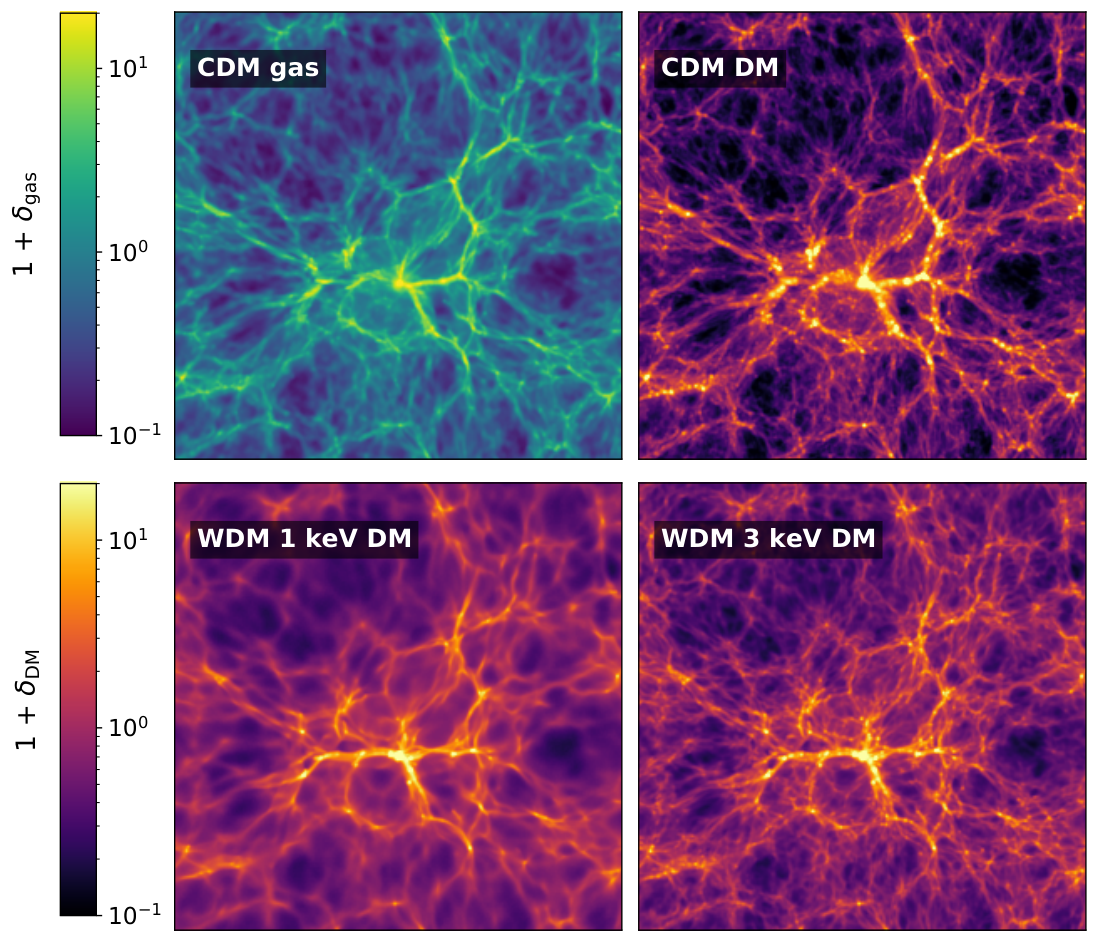
\includegraphics[width=0.85\textwidth,height=0.6\textheight,keepaspectratio]{fig-7.png}
\caption{Figure 1: Slice through a cosmological simulation of size 20 h\textasciicircum{}\{-1\} Mpc with 2 \textbackslash{}times 10243 dark matter (DM) and gas particles at z = 4.2 from the Sherwood-Relics simulation suite that was run with the P-Gadget3 code. Top panel: Hydrogen gas distribution (left), dark matter distribution in the standard CDM model (right). Bottom panel: dark matter distribution in a 1 keV WDM model (left) compared to a 3 keV WDM model (right) with brighter colours indicating higher density. [arXiv:2504.06367] Reproduced from arXiv:2504.06367 (extracted with \texttt{get\_paper\_figures}).}
\label{fig:7}
\end{figure}

\begin{figure}[H]
\centering
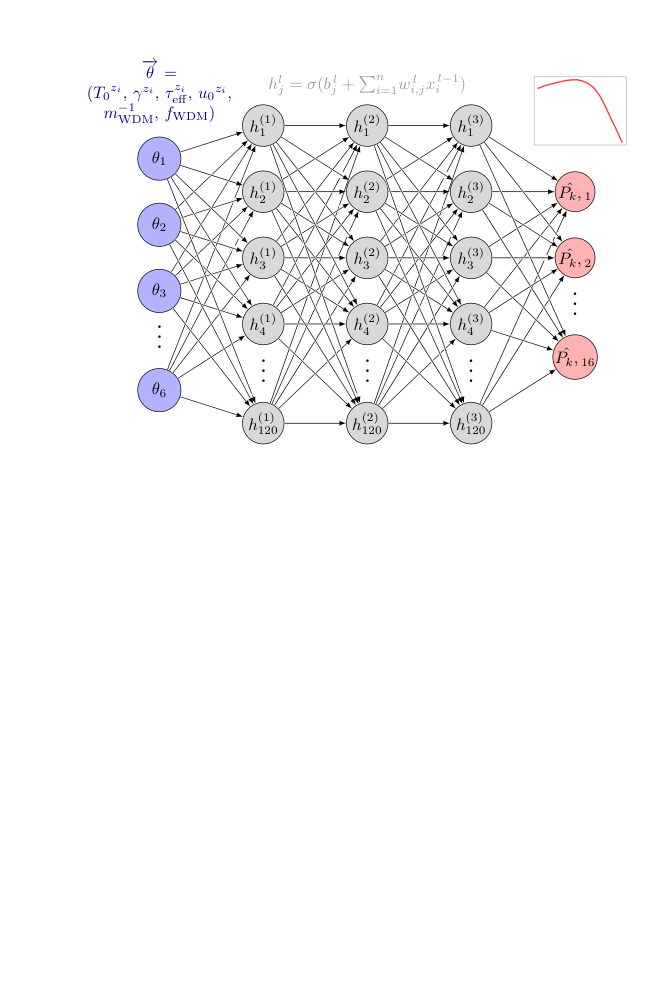
\includegraphics[width=0.85\textwidth,height=0.6\textheight,keepaspectratio]{fig-8.png}
\caption{Figure 4: Illustration of the emulator building process used in this work. Left: k-fold cross-validation. Right: Neural network trained on each fold i \textbackslash{}in [1,10]. We first extract the training set from the total input and output data to perform a k-fold cross-validation as shown on the left. Each fold is divided into 10 subsets, 9 are used to train the neural network model depicted on the right, while the remaining one is used as a validation set to monitor the convergence. We feed the cosmological model parameters \textbackslash{}overrightarrow\{\textbackslash{}theta\} in the input blue layer. The hidden layers are shown in [arXiv:2504.06367] Reproduced from arXiv:2504.06367 (extracted with \texttt{get\_paper\_figures}).}
\label{fig:8}
\end{figure}

\begin{figure}[H]
\centering
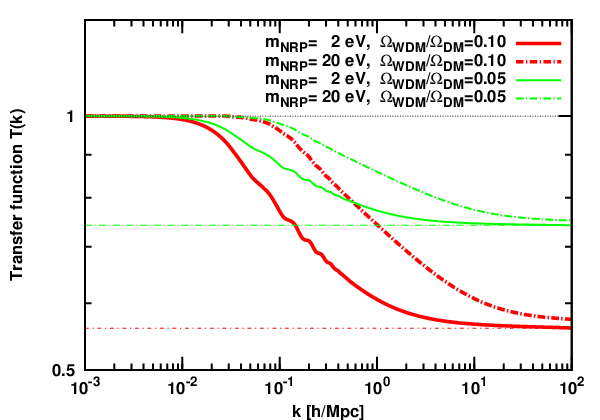
\includegraphics[width=0.85\textwidth,height=0.6\textheight,keepaspectratio]{fig-11.png}
\caption{Figure 2: The height of plateau in the transfer function T(k)\textbackslash{}equiv\textbackslash{}left[\{P\_\{\textbackslash{}Lambda\{\textbackslash{}textsc\{cwdm\}\}\}(k)\}/\{P\_\{\textbackslash{}Lambda\{\textbackslash{}textsc\{cdm\}\}\}(k)\}\textbackslash{}right]\textasciicircum{}\{1/2\} depends only on f\_\{\textbackslash{}textsc\{wdm\}\} only and does not change with the mass. In these examples, the mass is equal to 2\textbackslash{},\textbackslash{}\textgreater{}\textbackslash{}mathrm\{eV\} (solid line) or 20\textbackslash{},\textbackslash{}\textgreater{}\textbackslash{}mathrm\{eV\} (dashed-dotted line), while \textbackslash{}Omega\_\{\textbackslash{}textsc\{wdm\}\}/(\textbackslash{}Omega\_\{\textbackslash{}textsc\{wdm\}\}+\textbackslash{}Omega\_\{\textbackslash{}textsc\{cdm\}\})=0.1 (red) or 0.05 (green). Other parameters are fixed to \textbackslash{}Omega\_\{\textbackslash{}textsc\{b\}\}=0.05, \textbackslash{}Omega\_\{\textbackslash{}textsc\{m\}\}=0.3, \textbackslash{}Omega\_\{\textbackslash{}Lambda\}=0.7, h=0.7. [arXiv:0812.0010] Reproduced from arXiv:0812.0010 (extracted with \texttt{get\_paper\_figures}).}
\label{fig:11}
\end{figure}

\begin{figure}[H]
\centering
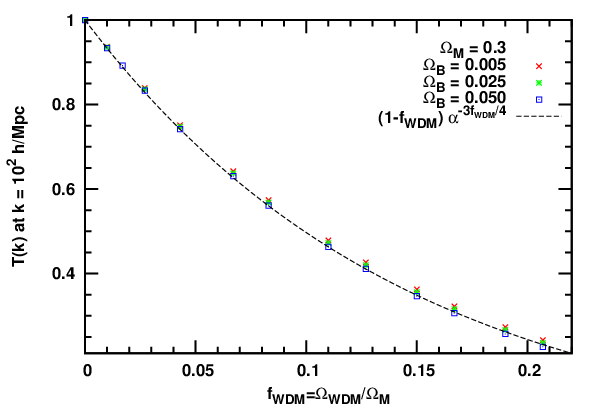
\includegraphics[width=0.85\textwidth,height=0.6\textheight,keepaspectratio]{fig-12.png}
\caption{Figure 3: Suppression factor T\_\{\textbackslash{}mathrm\{plateau\}\}=[\{P\_\{\textbackslash{}Lambda\{\textbackslash{}textsc\{cwdm\}\}\}(k)\}/\{P\_\{\textbackslash{}Lambda\{\textbackslash{}textsc\{cdm\}\}\}(k)\}]\textasciicircum{}\{1/2\} computed today at k=10\textasciicircum{}\{2\}\textbackslash{}\textgreater{}h/\textbackslash{}mathrm\{Mpc\} with the Boltzmann code CAMB, for different values of \{f\_\{\textbackslash{}textsc\{wdm\}\}\}\textbackslash{}equiv\textbackslash{}Omega\_\{\textbackslash{}textsc\{wdm\}\}/\textbackslash{}Omega\_\{\textbackslash{}textsc\{m\}\} and \textbackslash{}Omega\_\{\textbackslash{}textsc\{b\}\}. Other parameters are kept fixed: \textbackslash{}Omega\_\{\textbackslash{}Lambda\}=0.7, \textbackslash{}Omega\_\{\textbackslash{}textsc\{m\}\}=0.3, h=0.7. The dashed curve corresponds to the analytic prediction of Eq. (25) with \textbackslash{}alpha\textbackslash{}equiv\{a\_\{0\}g(a\_\{0\})\}/\{a\_\{\textbackslash{}mathrm\{eq\}\}\}=2.75\textbackslash{}times 10\textasciicircum{}\{3\}. [arXiv:0812.0010] Reproduced from arXiv:0812.0010 (extracted with \texttt{get\_paper\_figures}).}
\label{fig:12}
\end{figure}

\begin{figure}[H]
\centering
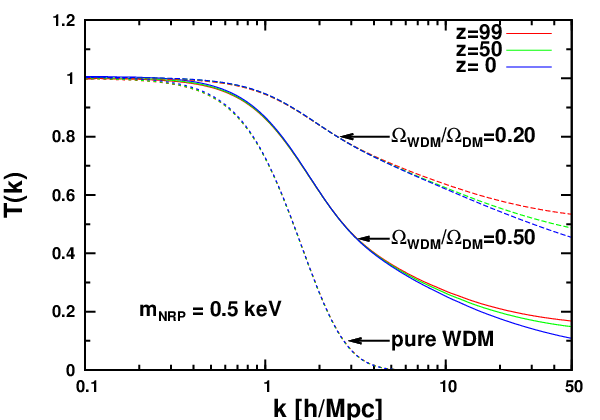
\includegraphics[width=0.85\textwidth,height=0.6\textheight,keepaspectratio]{fig-13.png}
\caption{Figure 4: Variation of T(k)=[\{P\_\{\textbackslash{}Lambda\{\textbackslash{}textsc\{cwdm\}\}\}(k)\}/\{P\_\{\textbackslash{}Lambda\{\textbackslash{}textsc\{cdm\}\}\}(k)\}]\textasciicircum{}\{1/2\} with redshift, for various values of m and \textbackslash{}Omega\_\{\textbackslash{}textsc\{wdm\}\}/(\textbackslash{}Omega\_\{\textbackslash{}textsc\{wdm\}\}+\textbackslash{}Omega\_\{\textbackslash{}textsc\{cdm\}\}); other parameters are fixed to the same values as in previous figures. (Left) For m=0.5\textasciitilde{}\textbackslash{}mathrm\{keV\}, the variation is clearly visible at large k\textgreater{}k\_\{\textbackslash{}textsc\{fs\}\}(z). (Right) For m=5\textasciitilde{}\textbackslash{}mathrm\{keV\}, the free-streaming wavenumber is too large for any variation to be seen on the scales displayed here. [arXiv:0812.0010] Reproduced from arXiv:0812.0010 (extracted with \texttt{get\_paper\_figures}).}
\label{fig:13}
\end{figure}

\begin{figure}[H]
\centering
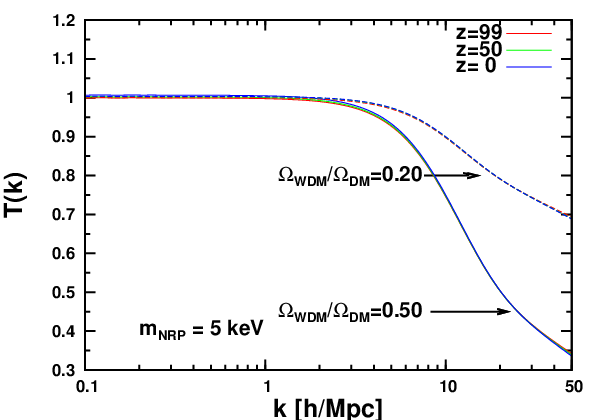
\includegraphics[width=0.85\textwidth,height=0.6\textheight,keepaspectratio]{fig-14.png}
\caption{Figure 4: Variation of T(k)=[\{P\_\{\textbackslash{}Lambda\{\textbackslash{}textsc\{cwdm\}\}\}(k)\}/\{P\_\{\textbackslash{}Lambda\{\textbackslash{}textsc\{cdm\}\}\}(k)\}]\textasciicircum{}\{1/2\} with redshift, for various values of m and \textbackslash{}Omega\_\{\textbackslash{}textsc\{wdm\}\}/(\textbackslash{}Omega\_\{\textbackslash{}textsc\{wdm\}\}+\textbackslash{}Omega\_\{\textbackslash{}textsc\{cdm\}\}); other parameters are fixed to the same values as in previous figures. (Left) For m=0.5\textasciitilde{}\textbackslash{}mathrm\{keV\}, the variation is clearly visible at large k\textgreater{}k\_\{\textbackslash{}textsc\{fs\}\}(z). (Right) For m=5\textasciitilde{}\textbackslash{}mathrm\{keV\}, the free-streaming wavenumber is too large for any variation to be seen on the scales displayed here. [arXiv:0812.0010] Reproduced from arXiv:0812.0010 (extracted with \texttt{get\_paper\_figures}).}
\label{fig:14}
\end{figure}

\begin{figure}[H]
\centering
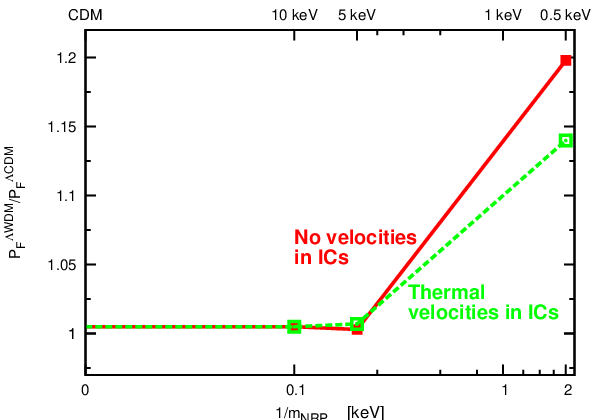
\includegraphics[width=0.85\textwidth,height=0.6\textheight,keepaspectratio]{fig-15.png}
\caption{Figure 5: Dependence of the flux PS of \textbackslash{}LambdaWDM models (divided by that of \textbackslash{}LambdaCDM) on thermal velocities in hydrodynamical simulations. The points show P\_\{F\}\textasciicircum{}\{\textbackslash{}Lambda\textbackslash{}mathrm\{WDM\}\}/P\_\{F\}\textasciicircum{}\{\textbackslash{}Lambda\textbackslash{}mathrm\{CDM\}\} at k=0.14\textbackslash{}\textgreater{}h/\textbackslash{}mathrm\{Mpc\} and z=2.2, extracted from GADGET-II simulations for three different masses, with and without thermal velocities in the initial conditions. The lines are the results of linear interpolation between these points. [arXiv:0812.0010] Reproduced from arXiv:0812.0010 (extracted with \texttt{get\_paper\_figures}).}
\label{fig:15}
\end{figure}

\begin{figure}[H]
\centering
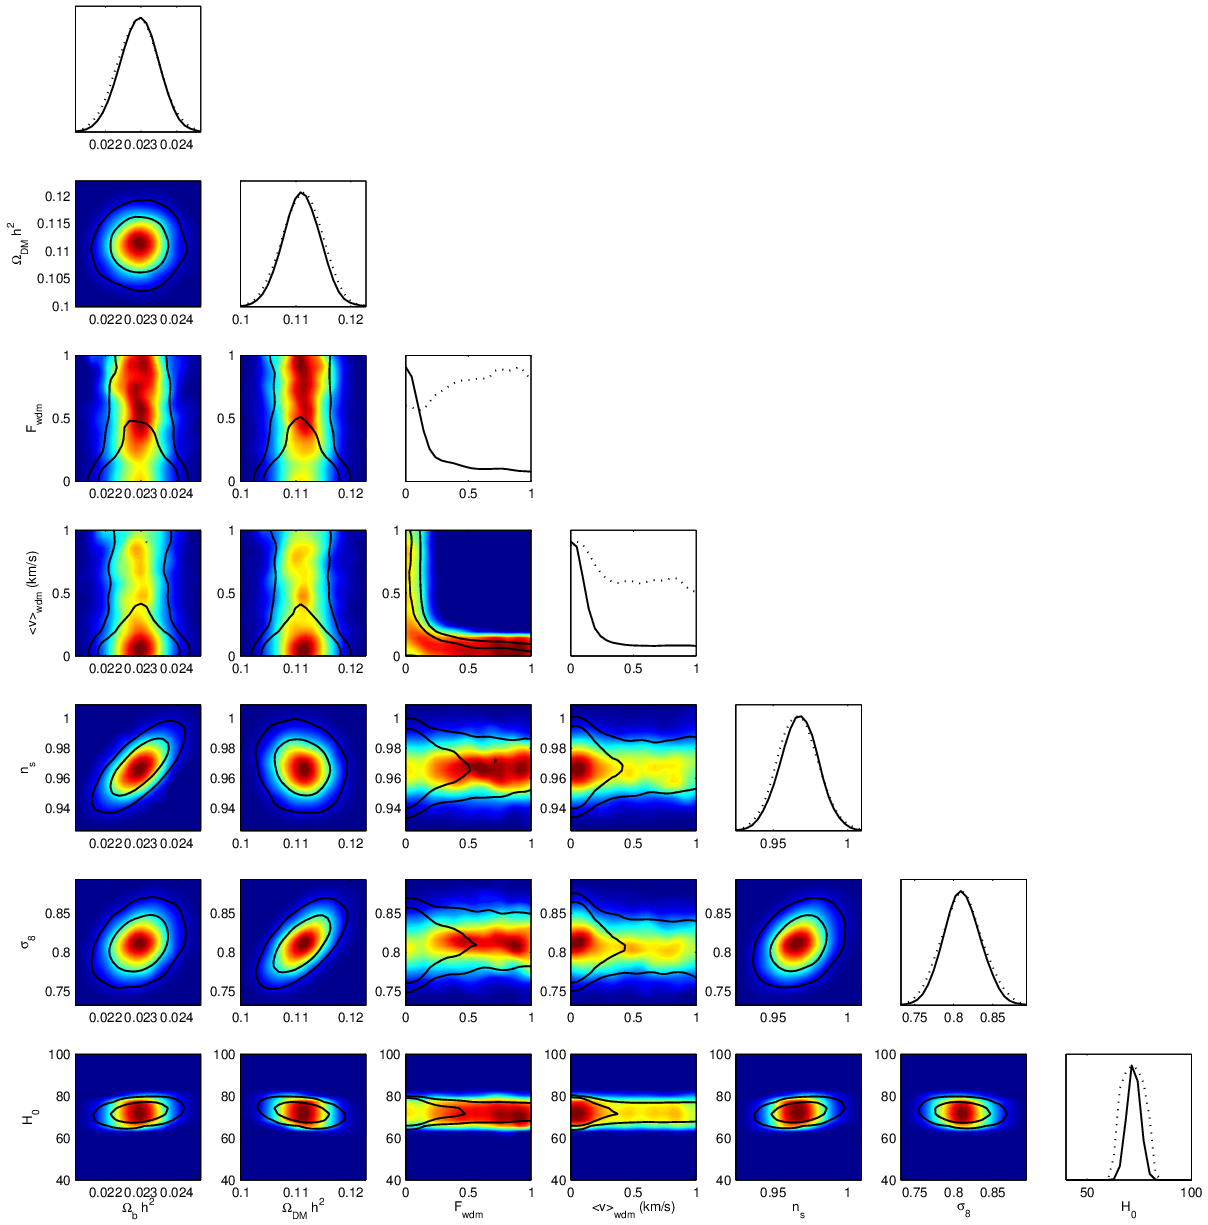
\includegraphics[width=0.85\textwidth,height=0.6\textheight,keepaspectratio]{fig-16.png}
\caption{Figure 6: Preferred region for pairs of cosmological parameters in the \textbackslash{}LambdaCWDM model, using VHS, WMAP5 and other cosmological data sets. The black lines represent the 68\textbackslash{}\%CL and 95\textbackslash{}\%CL contours of the two-dimensional probability marginalized over other parameters (as defined in the Bayesian approach), while the colors show the likelihood averaged over other parameters. The first five parameters \textbackslash{}Omega\_\{\textbackslash{}textsc\{b\}\}h\textasciicircum{}\{2\}, \textbackslash{}Omega\_\{\textbackslash{}textsc\{dm\}\}h\textasciicircum{}\{2\}, F\_\{\textbackslash{}textsc\{wdm\}\}, \textbackslash{}langle v\textbackslash{}rangle\_\{\textbackslash{}textsc\{wdm\}\}, n\_\{s\} have flat priors over the displayed range. Our analysis also assumes flat priors on the  [arXiv:0812.0010] Reproduced from arXiv:0812.0010 (extracted with \texttt{get\_paper\_figures}).}
\label{fig:16}
\end{figure}

\begin{figure}[H]
\centering
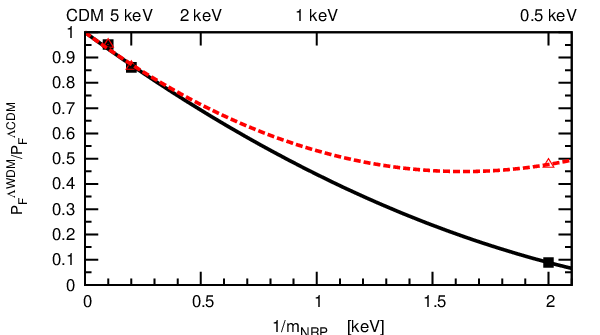
\includegraphics[width=0.85\textwidth,height=0.6\textheight,keepaspectratio]{fig-18.png}
\caption{Figure 8: Dependence of the interpolated flux PS of \textbackslash{}LambdaWDM models (divided by that of \textbackslash{}LambdaCDM) on thermal velocities in ICs, here for k=0.018s/km and z=4.2. The points are obtained with hydrodynamical simulations; the curves correspond to a global quadratic fit of these points. [arXiv:0812.0010] Reproduced from arXiv:0812.0010 (extracted with \texttt{get\_paper\_figures}).}
\label{fig:18}
\end{figure}

\begin{figure}[H]
\centering
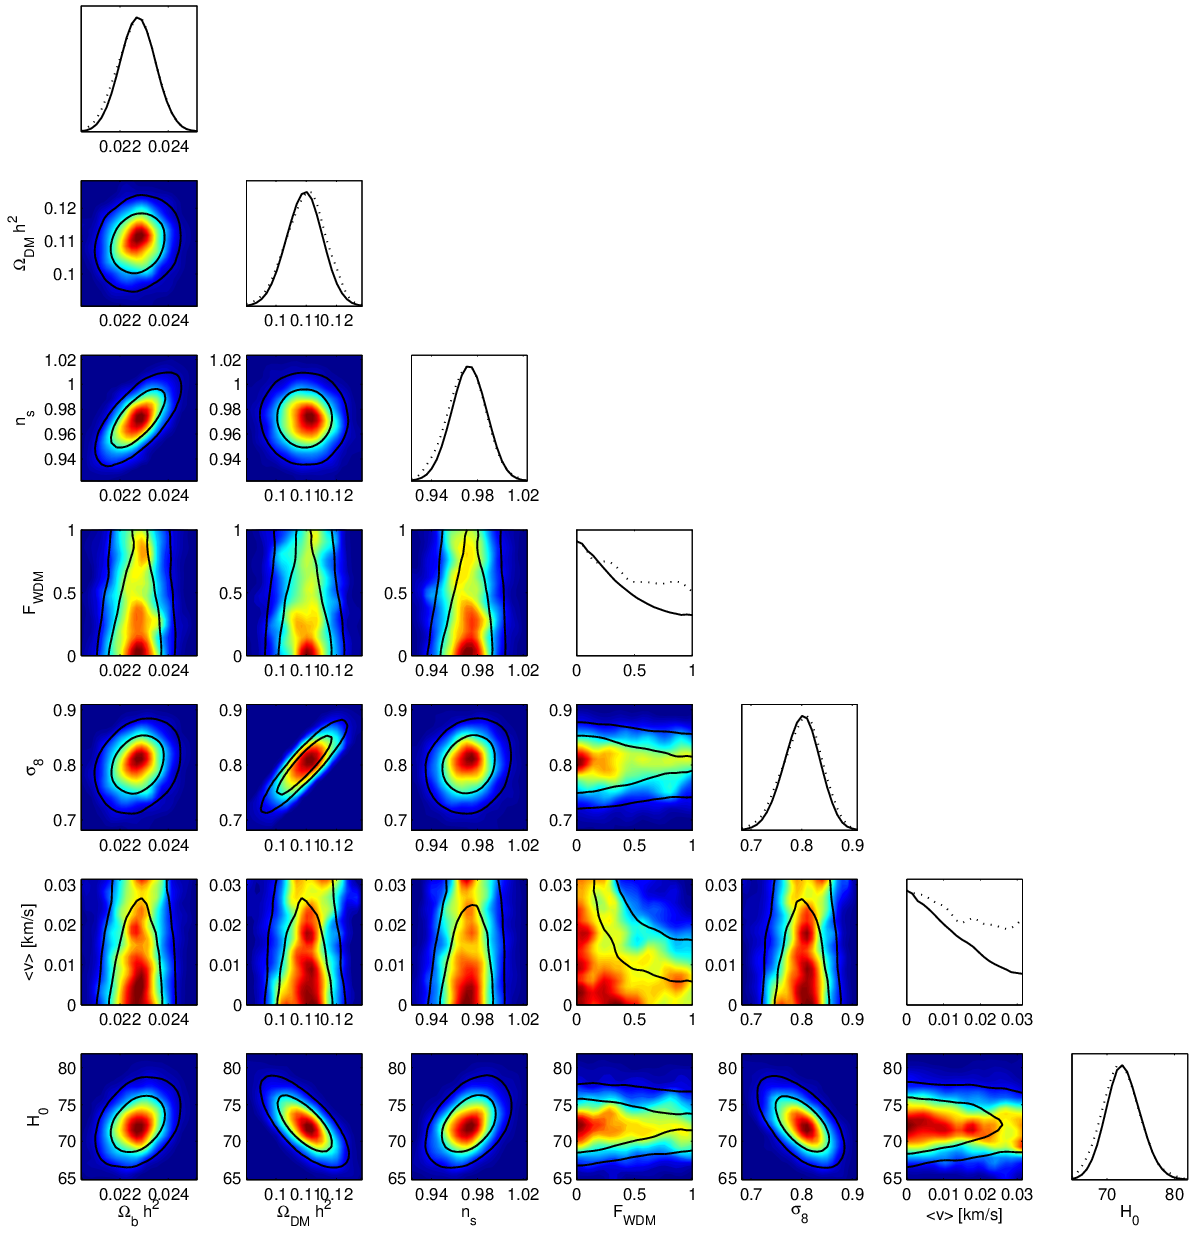
\includegraphics[width=0.85\textwidth,height=0.6\textheight,keepaspectratio]{fig-21.png}
\caption{Figure 11: Preferred region for pairs of cosmological parameters in the \textbackslash{}LambdaCWDM model, using SDSS Ly-\textbackslash{}alpha and WMAP5 data sets. The black lines represent the 68\textbackslash{}\%CL and 95\textbackslash{}\%CL contours of the two-dimensional probability marginalized over other parameters (as defined in the Bayesian approach), while the colors show the likelihood averaged over other parameters. The five parameters \textbackslash{}Omega\_\{\textbackslash{}textsc\{b\}\}h\textasciicircum{}\{2\}, \textbackslash{}Omega\_\{\textbackslash{}textsc\{dm\}\}h\textasciicircum{}\{2\}, n\_\{s\}, F\_\{\textbackslash{}textsc\{wdm\}\}, \textbackslash{}langle v\textbackslash{}rangle\_\{\textbackslash{}textsc\{wdm\}\} have flat priors over the displayed range. Our analysis also assumes flat priors on the logarithm of t [arXiv:0812.0010] Reproduced from arXiv:0812.0010 (extracted with \texttt{get\_paper\_figures}).}
\label{fig:21}
\end{figure}

\end{document}
